%! TeX root = dissertation.tex

\chapter{Dyadic Kernel Density Estimators}
\label{cha:kernel}

% abstract
Dyadic data is often encountered when quantities of interest are associated
with the edges of a network. As such it plays an important role in statistics,
econometrics and many other data science disciplines. We consider the problem
of uniformly estimating a dyadic Lebesgue density function, focusing on
nonparametric kernel-based estimators taking the form of dyadic empirical
processes. Our main contributions include the minimax-optimal uniform
convergence rate of the dyadic kernel density estimator, along with strong
approximation results for the associated standardized and Studentized
$t$-processes. A consistent variance estimator enables the construction of
valid and feasible uniform confidence bands for the unknown density function.
We showcase the broad applicability of our results by developing novel
counterfactual density estimation and inference methodology for dyadic data,
which can be used for causal inference and program evaluation. A crucial
feature of dyadic distributions is that they may be ``degenerate'' at certain
points in the support of the data, a property making our analysis somewhat
delicate. Nonetheless our methods for uniform inference remain robust to the
potential presence of such points. For implementation purposes, we discuss
inference procedures based on positive semi-definite covariance estimators,
mean squared error optimal bandwidth selectors and robust bias correction
techniques. We illustrate the empirical finite-sample performance of our
methods both in simulations and with real-world trade data, for which we make
comparisons between observed and counterfactual trade distributions in
different years. Our technical results concerning strong approximations and
maximal inequalities are of potential independent interest.

\section{Introduction}
\label{sec:introduction}

Dyadic data, also known as graphon data,
plays an important role in the statistical, social,
behavioral and biomedical sciences.
In network settings,
this type of dependent data captures
interactions between the units of study,
and its analysis is
of interest in statistics \citep{kolaczyk2009statistical}, economics
\citep{graham2020network}, psychology \citep{kenny2020dyadic}, public health
\citep{luke2007network} and many other data science disciplines.
For $n \geq 2$, a dyadic data set contains
$\frac{1}{2}n(n-1)$
observed real-valued random variables
%
\begin{align*}
  \bW_n = (W_{i j}:1\leq i<j \leq n),
  \quad\qquad W_{i j}
  &= W(A_i,A_j,V_{i j}),
\end{align*}
%
where $W$ is an unknown function, $\bA_n=(A_{i}:1\leq i \leq n)$
are independent and identically distributed (i.i.d.)\ latent random variables,
and $\bV_n=(V_{i j}:1\leq i<j \leq n)$ are i.i.d.\
latent random variables independent of $\bA_n$.
A natural interpretation of
this data is as a complete
undirected network on $n$ vertices,
with the latent variable $A_i$ associated with node $i$
and the observed variable $W_{i j}$ associated
with the edge between nodes $i$ and $j$.
The data generating process above is justified
without loss of generality by the celebrated
Aldous--Hoover representation theorem
for exchangeable arrays
\citep{aldous1981representations, hoover1979relations}.

Various distributional features of dyadic data are of interest in applications.
Most of the statistical literature focuses on parametric analysis, almost
exclusively considering moments of (transformations of)
the identically distributed $W_{i j}$.
See \citet{davezies2021exchangeable}, \citet{gao2021minimax},
\citet{MatsushitaOtsu2021}, and references therein, for contemporary
contributions and overviews. More recently, however, a few nonparametric
procedures for dyadic data have been proposed in the literature
\citep{graham2021dyadicregression,graham2022kernel}.

With the aim of estimating density-like functions
associated with $W_{i j}$ using
nonparametric kernel-based methods,
we investigate the statistical properties of a class
of local stochastic processes given by
%
\begin{align}\label{eq:kernel_estimator}
  w \mapsto \hat{f}_W(w)
  = \frac{2}{n(n-1)} \sum_{i=1}^{n-1} \sum_{j=i+1}^n k_h(W_{i j},w),
\end{align}
%
where $k_h(\cdot,w)$ is a kernel function
that can change with the $n$-varying bandwidth parameter
$h=h(n)$ and the evaluation point
$w \in \cW\subseteq \R$. For each $w\in\cW$ and with an appropriate choice of
the kernel function
(e.g.\ $k_h(\cdot,w)=K((\cdot-w)/h)/h$ for an interior point $w$
of $\cW$ and a fixed symmetric integrable kernel function $K$),
the statistic $\hat{f}_W(w)$ becomes a kernel density estimator
for the Lebesgue density function
$f_W(w) = \E\big[f_{W \mid AA}(w \mid A_i,A_j)\big]$,
where $f_{W \mid AA}(w \mid A_i,A_j)$ denotes the conditional Lebesgue density
of $W_{i j}$ given $A_i$ and $A_j$.
Setting
$k_h(\cdot,w)=K((\cdot-w)/h)/h$, \citet{graham2022kernel}
recently introduced the dyadic point estimator $\hat{f}_W(w)$ and studied
its large sample properties pointwise in $w\in\cW=\mathbb{R}$, while
\citet{chiang2020empirical} established its rate of convergence uniformly in
$w\in\cW$ for a compact interval $\cW$ strictly contained in the support of
the dyadic data $W_{i j}$.
\citet{chiang2022inference} obtained a distributional approximation for the
supremum statistic $\sup_{w\in\cW}\big|\hat{f}_W(w)\big|$
over a finite collection $\cW$ of design points.
More generally, as we discuss below,
the estimand $f_W(w)$ is useful in
different applications because it forms the basis for
counterfactual distributional analysis
(Section~\ref{sec:counterfactual})
and other nonparametric and semiparametric methods
(Section~\ref{sec:future}).
We remark that while we assume throughout that the network is complete,
our approach generalizes in a straightforward way to networks
with missing edges, as in Section~\ref{sec:trade_data}.
This can be seen by setting $W_{i j} = -\infty$
whenever the edge $\{i, j\}$ is not present, so that the law of
$W_{i j}$ is a mixture between a continuous distribution and a point mass
at $-\infty$.
We then apply our methodology to recover the
continuous component of this distribution,
following \citet{chiang2022inference}.

We contribute to the emerging
literature on nonparametric smoothing methods
for dyadic data with two main technical
results. Firstly, we derive the minimax rate of uniform convergence for density
estimation with dyadic data and show that the estimator
$\hat{f}_W$ in \eqref{eq:kernel_estimator}
is minimax-optimal under appropriate conditions.
Secondly, we present a set of
uniform distributional approximation results
for the \emph{entire} stochastic process $\big(\hat{f}_W(w):w\in\cW\big)$.
Furthermore, we illustrate the usefulness of our main results
with two distinct substantive statistical applications:
%
\begin{inlineroman}
\item
  confidence bands for $f_W$
  (Section~\ref{sec:implementation}), and
\item
  estimation and inference for counterfactual
  dyadic distributions (Section~\ref{sec:counterfactual}).
\end{inlineroman}
%
Our main results also lay the
foundation for studying the uniform distributional properties of other
nonparametric and semiparametric tests and estimators based on
dyadic data (Section~\ref{sec:future}).
Importantly, our inference
results cannot be deduced from the existing U-statistic, empirical process and
U-process theory available in the literature
\citep{van1996weak,gine2021mathematical} because,
as explained in detail below,
$\hat{f}_W(w)$ is not a standard U-statistic,
nor is the stochastic process $\hat{f}_W$ Donsker in general,
and the underlying dyadic data $\bW_n$ exhibits
statistical dependence due to its network structure.

Section~\ref{sec:kernel_setup} outlines the setup and presents the main
assumptions
imposed throughout the paper. We first discuss a Hoeffding-type decomposition of
the U-statistic-like $\hat{f}_W$ which is more general than the standard
Hoeffding decomposition for second-order U-statistics due
to its dyadic data structure.
In particular,
\eqref{eq:h-decomposition} shows that $\hat{f}_W(w)$ decomposes into a sum
of the four terms $B_n(w)$, $L_n(w)$, $E_n(w)$ and $Q_n(w)$,
where $E_n(w)$ is not present in the classical second-order U-statistic theory.
The first term $B_n(w)$ captures the usual smoothing bias, the second term
$L_n(w)$ is akin to the H\'{a}jek projection for second-order U-statistics, the
third term $E_n(w)$ is a mean-zero double
average of conditionally independent terms,
and the fourth term $Q_n(w)$ is a negligible totally degenerate
second-order U-process.
The leading stochastic
fluctuations of the process $\hat{f}_W$
are captured by $L_n$ and $E_n$,
both of which are known to be asymptotically distributed
as Gaussian random variables pointwise in $w\in\cW$ \citep{graham2022kernel}.
However, the H\'{a}jek projection term $L_n$ will often
be ``degenerate'' at some
or possibly all evaluation points $w\in\cW$.

Section~\ref{sec:point_estimation} studies minimax convergence rates for point
estimation of $f_W$ uniformly over $\cW$ and gives precise conditions under
which the estimator $\hat{f}_W$ is minimax-optimal.
Firstly, in Theorem~\ref{thm:uniform_consistency} we establish the uniform rate
of convergence of $\hat{f}_W$ for $f_W$. This result improves upon the
recent paper of \citet{chiang2020empirical} by allowing
for compactly supported dyadic data and
generic kernel-like functions $k_h$ (including boundary-adaptive kernels), while
also explicitly accounting for possible degeneracy of the
H\'{a}jek projection term $L_n$ at some or possibly all points $w\in\cW$.
Secondly, in Theorem~\ref{thm:kernel_minimax} we derive the
minimax uniform convergence rate for estimating
$f_W$, again allowing for possible degeneracy,
and verify that it is achieved by $\hat f_W$.
This result appears to be new to the literature,
complementing recent work on parametric moment estimation
using graphon data \citep{gao2021minimax} and on nonparametric
kernel-based regression using dyadic data \citep{graham2021dyadicregression}.

Section~\ref{sec:kernel_inference} presents a distributional analysis of
the stochastic process $\hat{f}_W$ uniformly in $w \in \cW$. Because
$\hat{f}_W$ is not asymptotically tight in general, it
does not converge
weakly in the space of uniformly bounded real functions supported on $\cW$ and
equipped with the uniform norm \citep{van1996weak},
and hence is non-Donsker.
To circumvent this problem,
we employ strong approximation methods to characterize
its distributional properties.
Up to the smoothing bias term $B_n$ and the negligible term $Q_n$,
it is enough to consider
the stochastic process $w \mapsto L_n(w)+E_n(w)$.
Since $L_n$ can be degenerate at some or possibly all points $w\in\cW$, and also
because under some bandwidth choices both $L_n$ and $E_n$ can be of comparable
order, it is crucial to analyze the joint distributional properties of $L_n$ and
$E_n$. To do so, we employ a carefully crafted conditioning approach where we
first establish an unconditional strong approximation for $L_n$ and a
conditional-on-$\bA_n$ strong approximation for $E_n$.
We then combine these to obtain a strong approximation for $L_n+E_n$.

The stochastic process $L_n$ is an empirical process indexed by an $n$-varying
class of functions depending only on the i.i.d.\ random variables $\bA_n$. Thus
we use the celebrated Hungarian
construction \citep{komlos1975approximation}, building on ideas in
\citet{gine2004kernel} and \citet{gine2010confidence}. The resulting rate of
strong approximation is optimal, and follows from a generic strong approximation
result of potential independent interest given in
Section~SA3 of
the online supplemental appendix.
Our main result for $L_n$ is given as Lemma~\ref{lem:strong_approx_Ln},
and makes explicit the potential presence of degenerate points.

The stochastic process $E_n$ is an empirical process depending on the dyadic
variables $W_{i j}$ and indexed by an $n$-varying class of functions.
When conditioning on $\bA_n$, the variables $W_{i j}$ are independent but not
necessarily identically distributed (i.n.i.d.), and thus we establish a
conditional-on-$\bA_n$ strong
approximation for $E_n$ based on the Yurinskii coupling
\citep{yurinskii1978error}, leveraging a recent refinement obtained by
\citet*[Lemma~38]{belloni2019conditional}.
This result follows from a generic
strong approximation result which
gives a novel rate of strong approximation for
(local) empirical processes based on i.n.i.d. data,
given in
Section~SA3 of
the online supplemental appendix.
Lemma~\ref{lem:conditional_strong_approx_En}
gives our conditional strong approximation for $E_n$.

Once the unconditional strong approximation for $L_n$ and the
conditional-on-$\bA_n$ strong approximation for $E_n$ are established,
we show how to properly ``glue'' them together to deduce a final unconditional
strong approximation for $L_n+E_n$ and hence also for $\hat{f}_W$ and its
associated $t$-process. This final step requires some additional technical work.
Firstly, building on our conditional strong approximation for $E_n$, we
establish an unconditional strong approximation for $E_n$ in
Lemma~\ref{lem:unconditional_strong_approx_En}. We then employ a
generalization of the celebrated Vorob'ev--Berkes--Philipp theorem
\citep{dudley1999uniform}, given in
Section~SA3 of
the online supplemental appendix,
to deduce a \emph{joint} strong
approximation for $(L_n,E_n)$ and, in particular, for $L_n+E_n$.
Thus we obtain our main result in Theorem~\ref{thm:strong_approx_fW},
which establishes a valid strong approximation for $\hat{f}_W$
and its associated $t$-process.
This uniform inference result complements the recent contribution of
\citet{davezies2021exchangeable}, which is not applicable
here because $\hat{f}_W$ is non-Donsker in general.

We illustrate the applicability of our strong approximation result for
$\hat{f}_W$ and its associated $t$-process by constructing valid
standardized uniform confidence bands for
the unknown density function $f_W$.
Instead of relying on extreme value theory \citep*[e.g.][]{gine2004kernel}, we
employ anti-concentration methods, following \citet{chernozhukov2014anti}.
This illustration improves on the recent work of \citet{chiang2022inference},
which obtained simultaneous confidence intervals for the dyadic density $f_W$
based on a high-dimensional central limit theorem over rectangles,
following prior work by \citet{Chernozhukov-Chetverikov-Kato_2017_AoP}.
The distributional
approximation therein is applied to the
H\'{a}jek projection term $L_n$ only, whereas
our main construction leading to Theorem~\ref{thm:strong_approx_fW} gives a
strong approximation for the entire U-process-like
$\hat{f}_W$ and its associated $t$-process, uniformly on $\cW$.
As a consequence, our uniform inference theory is robust to potential
unknown degeneracies in $L_n$ by virtue of our strong
approximation of $L_n+E_n$ and the use of proper standardization,
delivering a ``rate-adaptive'' inference procedure.
Our result appears to be the first to provide
confidence bands that are valid uniformly
over $w \in \cW$ rather than over some finite collection of design points.
Moreover, they provide distributional approximations for
the whole $t$-statistic process,
which can be useful in applications where functionals other
than the supremum are of interest.

Section~\ref{sec:implementation} addresses outstanding issues of
implementation. Firstly, we discuss estimation of the covariance function of the
Gaussian process underlying our strong approximation results. We present two
estimators, one based on the plug-in method, and the other based on a
positive semi-definite regularization thereof
\citep{laurent2005semidefinite}. We derive the uniform convergence rates for
both estimators in Lemma~\ref{lem:sdp}, which we then use to justify
Studentization of $\hat{f}_W$ and a
feasible simulation-based approximation of the infeasible Gaussian process
underlying our strong approximation results.
Secondly, we discuss integrated mean
squared error (IMSE) bandwidth selection and provide a simple rule-of-thumb
implementation for applications \citep{wand1994kernel,simonoff2012smoothing}.
Thirdly, we provide
feasible, valid uniform inference methods for
$f_W$ by employing robust bias correction
\citep{Calonico-Cattaneo-Farrell_2018_JASA,
Calonico-Cattaneo-Farrell_2022_Bernoulli}.
Algorithm~\ref{alg:method} summarizes our entire feasible methodology.

Section~\ref{sec:simulations} reports
empirical evidence for our proposed
feasible robust bias-corrected confidence bands for $f_W$.
We use simulations to show that these confidence bands are robust to potential
unknown degenerate points in the underlying dyadic distribution.

Section~\ref{sec:counterfactual} presents novel results for counterfactual
dyadic density estimation and inference,
offering an application of our general theory to a
substantive problem in statistics and other data science disciplines.
Counterfactual distributions are important for causal inference
and policy evaluation
\citep{dinardo1996distribution,chernozhukov2013inference},
and in the context of network data,
such analysis can be used to answer empirical questions
such as ``what would the international trade distribution in one year have been
if the gross domestic product (GDP) of the countries had
remained the same as in a previous year?''
We formally show how our theory for kernel-based dyadic estimators
can be used
to infer the counterfactual density function
of dyadic data had some monadic covariates followed a
different distribution.
We propose a two-step semiparametric reweighting approach in which we
first estimate the Radon--Nikodym derivative between the
observed and counterfactual
covariate distributions using a simple parametric estimator,
and then use this to construct a weighted dyadic kernel density estimator.
We present uniform consistency, strong approximation
and feasible inference results
for this dyadic counterfactual density estimator.
Finally, we also illustrate our methods
with a real dyadic data set recording bilateral trade between countries,
using GDP as a covariate for the counterfactual analysis.

Section~\ref{sec:future} discusses further statistical
applications of our main results,
including dyadic density hypothesis testing and nonparametric
and semiparametric dyadic regression.
Section~\ref{sec:conclusion} concludes the paper.
The online supplemental appendix includes other technical and methodological
results, proofs and additional details omitted here to conserve space.
Section~SA3 may be of independent interest, containing
two generic strong approximation theorems for empirical processes,
a generalized Vorob'ev--Berkes--Philipp theorem
and a maximal inequality for i.n.i.d.\ random variables.

\subsection{Notation}

The total variation norm of a
real-valued function $g$ of a single real variable is
written as
$\|g\|_\TV = \sup_{n \geq 1} \sup_{x_1 \leq \cdots \leq x_n}
\sum_{i=1}^{n-1} |g(x_{i+1}) - g(x_i)|$.
For an integer $m\geq 0$,
denote by $\mathcal{C}^m(\mathcal{X})$
the space of all $m$-times continuously differentiable functions
on $\mathcal{X}$.
For $\beta > 0$ and $C>0$,
define the H\"{o}lder class on $\mathcal{X}$ to be
\TODO{check this is correct}
$\cH^\beta_C(\cX)
=
\big\{
  g \in \cC^{\flbeta}(\cX): \
  \max_{1 \leq r \leq \flbeta}
  \big| g^{(r)}(x) \big| \leq C
  \text{ and }
  \big| g^{(\flbeta)}(x) - g^{(\flbeta)}(x') \big|
  \leq C |x-x'|^{\beta - \flbeta}, \
  \forall x, x' \in \cX
\big\},
$
where $\flbeta$ denotes the largest integer
which is strictly less than $\beta$.
For $a \in \R$ and $b \geq 0$,
we write $[a \pm b]$ for the interval $[a-b, a+b]$.
For non-negative sequences
$a_n$ and $b_n$, write
$a_n \lesssim b_n$ or $a_n = O(b_n)$
to indicate that
$a_n / b_n$ is bounded for $n\geq 1$.
Write $a_n \ll b_n$ or $a_n = o(b_n)$ if $a_n / b_n \to 0$.
If $a_n \lesssim b_n \lesssim a_n$,
write $a_n \asymp b_n$.
For random non-negative sequences
$A_n$ and $B_n$, write
$A_n \lesssim_\P B_n$ or $A_n = O_\P(B_n)$ if
$A_n / B_n$ is bounded in probability.
Write $A_n = o_\P(B_n)$ if $A_n / B_n \to 0$ in probability.
For $a,b \in \R$, define $a\wedge b=\min\{a,b\}$ and
$a \vee b = \max\{a,b\}$.

\section{Setup}\label{sec:kernel_setup}

We impose the following two assumptions throughout this paper.
%
\begin{assumption}[Data generation]\label{ass:kernel_data}\onehalfspacing
  %
  % A and V variables
  Let $\bA_n = (A_i: 1 \leq i \leq n)$ be i.i.d.\
  random variables supported on $\cA \subseteq \R$
  and let $\bV_n = (V_{i j}: 1 \leq i < j \leq n)$
  be i.i.d.\ random variables with a Lebesgue density $f_V$ on $\R$,
  with $\bA_n$ independent of $\bV_n$.
  %
  % W variables
  Let $W_{i j} = W(A_i, A_j, V_{i j})$
  and $\bW_n = (W_{i j}: 1 \leq i < j \leq n)$,
  where $W$ is an unknown real-valued function
  which is symmetric in its first two arguments.
  %
  Let $\cW \subseteq \R$ be a compact interval
  with positive Lebesgue measure $\Leb(\cW)$.
  The conditional distribution
  of $W_{i j}$ given $A_i$ and $A_j$
  admits a Lebesgue density $f_{W \mid AA}(w \mid A_i, A_j)$.
  For $\CH > 0$ and $\beta \geq 1$,
  take $f_W \in \cH^\beta_{\CH}(\cW)$ where
  $f_{W}(w) = \E\left[f_{W \mid AA}(w \mid A_i,A_j)\right]$
  and
  $f_{W \mid AA}(\cdot \mid a, a') \in \cH^1_{\CH}(\cW)$
  for all $a,a' \in \cA$.
  Suppose
  $\sup_{w \in \cW} \|f_{W \mid A}(w \mid \cdot\,)\|_\TV <\infty$ where
  $f_{W \mid A}(w \mid a) = \E\left[f_{W \mid AA}(w \mid A_i,a)\right]$.
  %
\end{assumption}

In Assumption~\ref{ass:kernel_data} we require
the density $f_W$ be in a $\beta$-smooth H\"older class of
functions on the compact interval $\cW$.
H\"older classes are well-established in the minimax estimation literature
\citep{gine2021mathematical}, with the smoothness parameter $\beta$ appearing
in the minimax-optimal rate of convergence.
If the H\"older condition is satisfied only piecewise,
then our results remain valid provided that the boundaries
between the pieces are known and treated as boundary points.

If $W(a_1, a_2, v)$ is strictly monotonic and continuously differentiable in
its third argument,
we can give the conditional density of $W_{i j}$ explicitly
using the usual change-of-variables formula: with $w=W(a_1,a_2,v)$,
we have
$f_{W \mid AA}(w \mid a_1,a_2) = f_V(v)
\big|\partial W(a_1,a_2,v)/\partial v\big|^{-1}$.

\begin{assumption}[Kernels and bandwidth]\label{ass:kernel_bandwidth}%
  \onehalfspacing

  Let $h = h(n) > 0$
  be a sequence of bandwidths
  satisfying $h \log n \to 0$
  and $\frac{\log n}{n^2h} \to 0$.
  For each $w \in \cW$, let $k_h(\cdot, w)$
  be a real-valued function supported on
  $[w \pm h] \cap \cW$.
  For an integer $p \geq 1$,
  let $k_h$ belong to a family of
  boundary bias-corrected kernels of order $p$, i.e.,
  %
  \begin{align*}
    \int_{\cW}
    (s-w)^r k_h(s,w) \diff{s}
    \quad
    \begin{cases}
      \begin{alignedat}{2}
        &= 1 &\qquad &\text{for all } w \in \cW \text{ if }\, r = 0, \\
        &= 0 & &\text{for all } w \in \cW \text{ if }\, 1 \leq r \leq p-1, \\
        &\neq 0 & &\text{for some } w \in \cW \text{ if }\, r = p.
      \end{alignedat}
    \end{cases}
  \end{align*}
  %
  Also, for $\CL > 0$,
  suppose $k_h(s, \cdot) \in \cH^1_{\CL h^{-2}}(\cW)$
  for all $s \in \cW$.
  %
\end{assumption}

This assumption allows for all standard compactly supported
and possibly boundary-corrected kernel functions
\citep{wand1994kernel,simonoff2012smoothing}.
Assumption~\ref{ass:kernel_bandwidth} implies that
if $h \leq 1$ then
$k_h$ is uniformly bounded by
$\Ck h^{-1}$ where $\Ck \vcentcolon = 2 \CL + 1 + 1/\Leb(\cW)$.

\subsection{Hoeffding-type decomposition and degeneracy}
\label{sec:degeneracy}

The estimator $\hat{f}_W(w)$ is akin to a
U-statistic and thus admits a Hoeffding-type decomposition
which is the starting point for our analysis. We have
%
\begin{align}\label{eq:h-decomposition}
  \hat{f}_W(w) - f_W(w) = B_n(w) + L_n(w) + E_n(w) + Q_n(w)
\end{align}
%
with
$B_n(w) = \E\big[\hat{f}_W(w)\big] - f_W(w)$
and
%
\begin{align*}
  L_n(w)
  &= \frac{2}{n} \sum_{i=1}^n l_i(w), \\
  E_n(w)
  &=
  \frac{2}{n(n-1)} \sum_{i=1}^{n-1} \sum_{j=i+1}^{n} e_{i j}(w), \\
  Q_n(w)
  &=
  \frac{2}{n(n-1)} \sum_{i=1}^{n-1} \sum_{j=i+1}^{n} q_{i j}(w),
\end{align*}
%
where
$l_i(w) = \E[k_h(W_{i j},w) \mid A_i] - \E[k_h(W_{i j},w)]$,
$e_{i j}(w) = k_h(W_{i j},w) - \E[k_h(W_{i j},w) \mid A_i, A_j]$
and
$q_{i j}(w) = \E[k_h(W_{i j},w) \mid A_i, A_j] - \E[k_h(W_{i j},w) \mid A_i]
- \E[k_h(W_{i j},w) \mid A_j] + \E[k_h(W_{i j},w)]$.
The non-random term $B_n$ captures the smoothing (or misspecification) bias,
while the three stochastic processes $L_n$, $E_n$ and $Q_n$
capture the variance of the estimator.
These processes are
mean-zero with $\E[L_n(w)] = \E[Q_n(w)] = \E[E_n(w)] = 0$ for all $w \in \cW$,
and mutually orthogonal in $L^2(\P)$ since
$\E[L_n(w) Q_n(w')] = \E[L_n(w) E_n(w')] = \E[Q_n(w) E_n(w')] = 0$
for all $w, w' \in \cW$.

The stochastic process $L_n$ is akin to the H\'{a}jek projection of a U-process,
which can (and often will) exhibit degeneracy at some
or possibly all points $w \in \cW$.
To characterize different types of degeneracy,
we introduce the following non-negative lower and upper degeneracy constants:
%
\[
  \Dl^2 := \inf_{w \in \cW} \Var\left[f_{W \mid A}(w \mid A_i)\right]
  \qquad \text{ and } \qquad
  \Du^2 := \sup_{w \in \cW} \Var\left[f_{W \mid A}(w \mid A_i)\right].
\]
%
The following lemma describes the stochastic order of
different terms in the Hoeffding-type decomposition,
explicitly accounting for potential degeneracy.

\begin{lemma}[Bias and variance] \label{lem:variance}
  Suppose Assumptions \ref{ass:kernel_data}~and~\ref{ass:kernel_bandwidth}
  hold. Then the bias satisfies
  $\sup_{w \in \cW} \big| B_n(w) \big| \lesssim h^{p\wedge\beta}$,
  and the variance terms satisfy
  %
  \begin{align*}
    \E\left[ \sup_{w \in \cW} |L_n(w)| \right]
    &\lesssim
    \frac{\Du}{\sqrt n},
    &
    \E\left[ \sup_{w \in \cW} |E_n(w)| \right]
    &\lesssim \sqrt{\frac{\log n}{n^2h}},
    &
    \E\left[ \sup_{w \in \cW} |Q_n(w)| \right]
    \lesssim \frac{1}{n}.
  \end{align*}
\end{lemma}

Lemma~\ref{lem:variance} captures the potential total degeneracy of $L_n$ by
showing that if
$\Du=0$ then $L_n=0$ everywhere on $\cW$ almost surely.
The following lemma
captures the potential partial degeneracy of $L_n$, where
$\Du > \Dl = 0$.
For $w,w' \in \cW$,
define the covariance function of the dyadic kernel density estimator as
%
\begin{equation*}
  \Sigma_n(w,w')
  =
  \E\Big[
    \Big(
      \hat f_W(w)
      - \E\big[\hat f_W(w)\big]
    \Big)
    \Big(
      \hat f_W(w')
      - \E\big[\hat f_W(w')\big]
    \Big)
  \Big].
\end{equation*}
%
\begin{lemma}[Variance bounds]
  \label{lem:variance_bounds}
  Suppose that Assumptions~\ref{ass:kernel_data}
  and~\ref{ass:kernel_bandwidth} hold.
  Then for sufficiently large $n$,
  %
  \begin{align*}
    \frac{\Dl^2}{n} + \frac{1}{n^2h}
    \inf_{w \in \cW} f_W(w)
    &\lesssim
    \inf_{w \in \cW} \Sigma_n(w,w)
    \leq
    \sup_{w \in \cW} \Sigma_n(w,w)
    \lesssim
    \frac{\Du^2}{n} + \frac{1}{n^2h}.
  \end{align*}
  %
\end{lemma}

Combining Lemmas~\ref{lem:variance} and~\ref{lem:variance_bounds},
we have the following trichotomy
for degeneracy of dyadic distributions
based on $\Dl$ and $\Du$:
%
\begin{inlineroman}
\item
  total degeneracy if $\Du = \Dl = 0$,
\item
  partial degeneracy if $\Du > \Dl = 0$,
\item
  no degeneracy if $\Dl > 0$.
\end{inlineroman}
%
In the case of no degeneracy,
it can be shown that
$\inf_{w \in \cW} \Var[L_n(w)] \gtrsim n^{-1}$,
while in the case of total degeneracy,
$L_n(w) = 0$ for all $w \in \cW$ almost surely.
When the dyadic distribution is partially degenerate,
there exists at least one point
$w\in\cW$ such that
$\Var\left[f_{W \mid A}(w \mid A_i)\right] = 0$
and $\Var[L_n(w)]\lesssim h n^{-1}$,
and there also exists at least one point
$w'\in \cW$ such that
$\Var\left[f_{W \mid A}(w' \mid A_i)\right] > 0$ and
$\Var[L_n(w')] \gtrsim \frac{1}{n}$.
We say $w$ is a \emph{degenerate point}
if $\Var\left[f_{W \mid A}(w \mid A_i)\right] = 0$,
and otherwise say it is a
\emph{non-degenerate point}.

As a simple example,
consider the family of dyadic distributions $\P_{\pi}$
indexed by $\pi = (\pi_1, \pi_2, \pi_3)$
with $\sum_{i=1}^3 \pi_i = 1$ and $\pi_i \geq 0$,
generated by $W_{i j} = A_i A_j + V_{i j}$,
where $A_i$ equals $-1$ with probability $\pi_1$,
equals $0$ with probability $\pi_2$
and equals $+1$ with probability $\pi_3$,
and $V_{i j}$ is standard Gaussian.
This model induces a latent
``community structure'' where community membership
is determined by the value of $A_i$ for each node $i$,
and the interaction outcome $W_{i j}$ is a function
only of the communities which $i$ and $j$ belong to and some
idiosyncratic noise.
Unlike the stochastic block model
\citep{kolaczyk2009statistical},
our setup assumes that
community membership has no impact on edge existence,
as we work with fully connected networks;
see Section~\ref{sec:trade_data} for a discussion of
how to handle missing edges in practice.
Also note that the parameter of interest in this paper is the Lebesgue density
of a continuous random variable $W_{i j}$
rather than the probability of network edge existence,
which is the focus of graphon estimation
literature \citep{gao2021minimax}.

In line with Assumption~\ref{ass:kernel_data}, $\bA_n$ and $\bV_n$ are i.i.d.\
sequences independent of each other.
Then
$f_{W \mid AA}(w \mid A_i, A_j) = \phi(w - A_i A_j)$,\,
$f_{W \mid A}(w \mid A_i) = \pi_1 \phi(w + A_i) + \pi_2 \phi(w)
+ \pi_3 \phi(w - A_i)$
and
$f_W(w) = (\pi_1^2 + \pi_3^2) \phi(w-1) + \pi_2 (2 - \pi_2) \phi(w) + 2
\pi_1 \pi_3 \phi(w+1),$
where $\phi$ denotes the probability density function of
the standard normal distribution.
Note that $f_W(w)$ is strictly positive for all $w \in \R$.
Consider the parameter choices:
%
\begin{enumerate}[label=(\roman*)]\onehalfspacing

  \item $\pi = \left( \frac{1}{2}, 0, \frac{1}{2} \right)$:\quad
    $\P_\pi$ is degenerate at all $w \in \R$,

  \item $\pi = \left( \frac{1}{4}, 0, \frac{3}{4} \right)$:\quad
    $\P_\pi$ is degenerate only at $w=0$,

  \item $\pi = \left( \frac{1}{5}, \frac{1}{5}, \frac{3}{5} \right)$:\quad
    $\P_\pi$ is non-degenerate for all $w \in \R$.

\end{enumerate}
%
Figure~\ref{fig:distribution} demonstrates these phenomena,
plotting the unconditional density $f_W$
and the standard deviation of the conditional density $f_{W|A}$
over $\cW = [-2,2]$ for each choice of the parameter $\pi$.

The trichotomy of total/partial/no  degeneracy is useful for understanding the
distributional properties of the dyadic kernel density estimator
$\hat{f}_W(w)$. Crucially, our need for uniformity in $w$ complicates the
simpler degeneracy/no degeneracy dichotomy observed previously in the literature
\citep{graham2022kernel}.
More specifically,
from a pointwise-in-$w$ perspective,
partial degeneracy causes no issues,
while it is a fundamental problem
when conducting inference uniformly over $w \in \cW$.
We develop inference methods
that are valid uniformly over $w \in \cW$,
regardless of the presence of partial or total degeneracy.

\begin{figure}[ht]
  \captionsetup[subfigure]{justification=centering}
  \centering
  %
  \begin{subfigure}{0.32\textwidth}
    \centering
    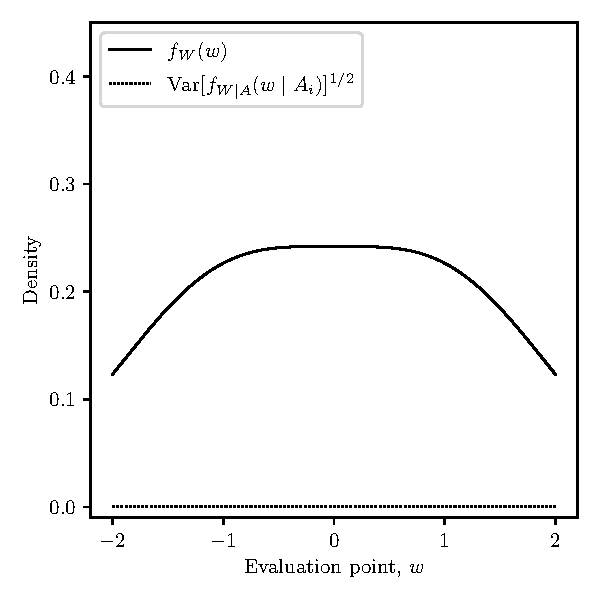
\includegraphics[scale=0.48]{graphics/illustration_total.pdf}
    \caption{
      Total degeneracy, \\
      $\pi = \left( \frac{1}{2}, 0, \frac{1}{2} \right)$
    }
  \end{subfigure}
  %
  \begin{subfigure}{0.32\textwidth}
    \centering
    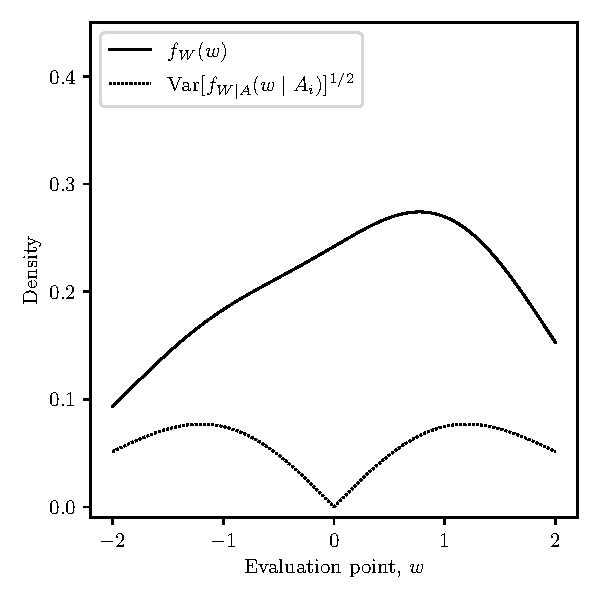
\includegraphics[scale=0.48]{graphics/illustration_partial.pdf}
    \caption{
      Partial degeneracy, \\
      $\pi = \left( \frac{1}{4}, 0, \frac{3}{4} \right)$
    }
  \end{subfigure}
  %
  \begin{subfigure}{0.32\textwidth}
    \centering
    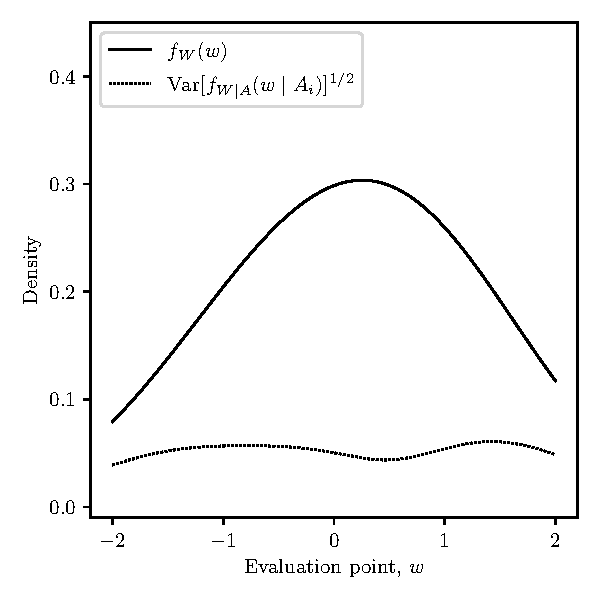
\includegraphics[scale=0.48]{graphics/illustration_none.pdf}
    \caption{
      No degeneracy, \\
      $\pi = \left( \frac{1}{5}, \frac{1}{5}, \frac{3}{5} \right)$
    }
  \end{subfigure}
  %
  \caption{
    Density $f_W$ and standard deviation
    of $f_{W|A}$ for the family of distributions $\P_\pi$.\\
  }
  %
  \label{fig:distribution}
\end{figure}

\section{Point estimation results}\label{sec:point_estimation}

Using Lemma~\ref{lem:variance},
the next theorem establishes the uniform
convergence rate of $\hat{f}_W$.
%
\begin{theorem}[Uniform convergence rate]%
  \label{thm:uniform_consistency}%
  Suppose that Assumptions
  \ref{ass:kernel_data}~and~\ref{ass:kernel_bandwidth}
  hold. Then
  %
  \begin{align*}
    \E\left[
      \sup_{w \in \cW}
      \big|\hat{f}_W(w) - f_W(w)\big|
    \right]
    \lesssim
    h^{p\wedge\beta}
    + \frac{\Du}{\sqrt n}
    + \sqrt{\frac{\log n}{n^2h}}.
  \end{align*}
\end{theorem}
%
The constant in Theorem~\ref{thm:uniform_consistency}
depends only on $\cW$, $\beta$, $\CH$
and the choice of kernel.
We interpret this result in light of the degeneracy trichotomy.
\begin{enumerate}[label=(\roman*)]\onehalfspacing
  \item Partial or no degeneracy:
    $\Du > 0$.
    Any bandwidths satisfying
    $n^{-1} \log n \lesssim h \lesssim n^{-\frac{1}{2(p\wedge\beta)}}$
    yield
    $\E\big[\sup_{w \in \cW}\big|\hat f_W(w)
    - f_W(w)\big| \big] \lesssim \frac{1}{\sqrt n}$,
    the ``parametric'' bandwidth-independent rate noted by
    \citet{graham2022kernel}.

  \item Total degeneracy:
    $\Du = 0$.
    Minimizing the bound in
    Theorem~\ref{thm:uniform_consistency} with
    $h \asymp \left( \frac{\log n}{n^2} \right)^{\frac{1}{2(p\wedge\beta)+1}}$
    yields
    $\E\big[ \sup_{w \in \cW} \big|\hat f_W(w) - f_W(w)\big| \big]
    \lesssim
    \big(\frac{\log n}{n^2} \big)^{\frac{p\wedge\beta}{2(p\wedge\beta)+1}}$.
\end{enumerate}

These results generalize \citet*[Theorem~1]{chiang2020empirical}
by allowing for compactly supported data and more general kernel-like
functions $k_h(\cdot,w)$, enabling boundary-adaptive density estimation.

\subsection{Minimax optimality}

We establish the minimax rate under the
supremum norm for density estimation
with dyadic data.
This implies minimax optimality of the kernel density estimator $\hat
f_W$, regardless of the degeneracy type of the dyadic distribution.

\begin{theorem}[Uniform minimax rate] \label{thm:kernel_minimax}

  Fix $\beta \geq 1$ and $\CH > 0$,
  and let $\cW$ be a compact interval with positive Lebesgue measure.
  Define $\cP = \cP(\cW, \beta, \CH)$
  as the class of dyadic distributions
  satisfying Assumption~\ref{ass:kernel_data}.
  Define $\cPd$ as the subclass of $\cP$
  containing only those dyadic distributions
  which are totally degenerate on $\cW$ in the sense that
  $\sup_{w \in \cW} \Var\left[f_{W \mid A}(w \mid A_i)\right] = 0$.
  Then
  $\inf_{\tilde f_W} \sup_{\P \in \cP}
  \E_\P\big[\sup_{w \in \cW} \big| \tilde f_W(w) - f_W(w) \big| \big]
  \asymp \frac{1}{\sqrt n}$
  and
  $\inf_{\tilde f_W} \sup_{\P \in \cPd}
  \E_\P\big[\sup_{w \in \cW} \big| \tilde f_W(w) - f_W(w) \big| \big]
  \asymp \big( \frac{\log n}{n^2} \big)^{\frac{\beta}{2\beta+1}}$,
  where $\tilde f_W$ is any estimator depending only on
  the data $\bW_n = (W_{i j}: 1 \leq i < j \leq n)$
  distributed according to the dyadic distribution $\P$.
  The constants underlying $\asymp$ depend only on
  $\cW$, $\beta$ and $\CH$.

\end{theorem}

Theorem~\ref{thm:kernel_minimax} shows that the uniform convergence rate of
$n^{-1/2}$
obtained in Theorem~\ref{thm:uniform_consistency}
(coming from the $L_n$ term) is minimax-optimal in general.
When attention is restricted to totally degenerate dyadic distributions,
$\hat f_W$ also achieves the minimax rate of uniform convergence
(assuming a kernel of sufficiently high order $p \geq \beta$),
which is on the order of
$\left(\frac{\log n}{n^2}\right)^{\frac{\beta}{2\beta+1}}$ and
is determined by the bias $B_n$ and the leading variance term $E_n$ in
\eqref{eq:h-decomposition}.

Combining Theorems \ref{thm:uniform_consistency}~and~\ref{thm:kernel_minimax},
we
conclude that $\hat{f}_W(w)$ achieves the minimax-optimal rate
of uniform convergence for estimating $f_W(w)$ if
$h \asymp \left( \frac{\log n}{n^2} \right)^{\frac{1}{2\beta+1}}$
and $p \geq \beta$,
whether or not there are
any degenerate points in the underlying data generating process.
This result appears to be new to the literature on
nonparametric estimation with dyadic data.
See \citet{gao2021minimax} for a contemporaneous review.

\section{Distributional results}\label{sec:kernel_inference}

We investigate the distributional properties of the
standardized $t$-statistic process
%
\[ T_n(w) = \frac{\hat{f}_W(w) - f_W(w)}{\sqrt{\Sigma_n(w,w)}}
, \qquad w\in\cW,\]
%
which is not necessarily asymptotically tight.
Therefore, to approximate the distribution of the entire $t$-statistic process,
as well as specific functionals thereof, we rely on a novel strong approximation
approach outlined in this section.
Our results can be used to perform valid uniform inference irrespective of the
degeneracy type.

This section is largely concerned with distributional properties and thus
frequently requires copies of stochastic processes.
For succinctness of notation, we will not differentiate between a process
and its copy, but details are available in
Section~SA3 of the supplemental appendix.

\subsection{Strong approximation}

By the Hoeffding-type decomposition
\eqref{eq:h-decomposition} and Lemma~\ref{lem:variance},
it suffices to consider the distributional properties
of the stochastic process $(L_n(w)+E_n(w):w\in\cW)$.
Our approach combines the K\'omlos--Major--Tusn\'ady (KMT) approximation
\citep{komlos1975approximation} to obtain a strong approximation of
$L_n$ with a Yurinskii approximation
\citep{yurinskii1978error} to obtain a
\emph{conditional} (on $\bA_n$) strong approximation of
$E_n$.
The latter is necessary because
$E_n$ is akin to a local empirical process of i.n.i.d.\
random variables, conditional on $\bA_n$,
and therefore the KMT approximation is not applicable.
These approximations are then combined to give a final
(unconditional) strong approximation for $L_n+E_n$,
and thus for the $t$-statistic process
$(T_n(w):w\in\cW)$.

The following lemma is an application of our generic
KMT approximation result for empirical processes,
given in Section~SA3 of
the online supplemental appendix,
which builds on earlier work by \citet{gine2004kernel}
and \citet{gine2010confidence} and may be of independent interest.

\begin{lemma}[Strong approximation of $L_n$]
  \label{lem:strong_approx_Ln}
  Suppose that Assumptions
  \ref{ass:kernel_data}~and~\ref{ass:kernel_bandwidth} hold.
  For each $n$ there exists
  a mean-zero Gaussian process
  $Z^L_n$ indexed on $\cW$ satisfying
  $\E\big[ \sup_{w \in \cW} \big| \sqrt{n} L_n(w) -  Z_n^L(w) \big| \big]
  \lesssim \frac{\Du \log n}{\sqrt{n}}$,
  where $\E[Z_n^L(w)Z_n^L(w')] =  n\E[L_n(w)L_n(w')]$ for all $w, w' \in \cW$.
  The process $Z_n^L$
  is a function only of $\bA_n$ and some random noise
  independent of $(\bA_n, \bV_n)$.
\end{lemma}

% donsker case
The strong approximation result in Lemma~\ref{lem:strong_approx_Ln} would be
sufficient to develop valid and even optimal
uniform inference procedures whenever
(i) $\Dl > 0$ (no degeneracy in $L_n$) and
(ii) $n h \gg \log n$ ($L_n$ is leading).
In this special case, the recent Donsker-type results of
\citet{davezies2021exchangeable}
can be applied to analyze the limiting distribution
of the stochastic process $\hat{f}_W$.
Alternatively,
again only when $L_n$ is non-degenerate and leading,
standard empirical process methods could also be used.
However, even in the special case when $\hat{f}_W(w)$ is asymptotically
Donsker, our result in Lemma~\ref{lem:strong_approx_Ln}
improves upon the literature by providing a rate-optimal strong approximation
for $\hat{f}_W$ as opposed to only a weak convergence result.
See Theorem \ref{thm:infeasible_ucb} and the subsequent
discussion below.

% however often non-donsker
More importantly, as illustrated above,
it is common in the literature to find dyadic
distributions which exhibit partial or total degeneracy, making the process
$\hat{f}_W$ non-Donsker.
Thus approximating only $L_n$ is in general insufficient
for valid uniform inference,
and it is necessary to capture the distributional properties of $E_n$ as well.
% we do better
The following lemma is an application of
our strong approximation result for
empirical processes based on the Yurinskii approximation,
which builds on a refinement by \citet{belloni2019conditional}.

\begin{lemma}[Conditional strong approximation of $E_n$]
  \label{lem:conditional_strong_approx_En}

  Suppose Assumptions
  \ref{ass:kernel_data}~and~\ref{ass:kernel_bandwidth} hold
  and take any $R_n \to \infty$.
  For each $n$ there exists
  $\tilde Z^E_n$
  which is a mean-zero Gaussian process
  conditional on $\bA_n$ satisfying
  $\sup_{w \in \cW}
  \big| \sqrt{n^2h} E_n(w) - \tilde Z_n^E(w) \big|
  \lesssim_\P \frac{(\log n)^{3/8} R_n}{n^{1/4}h^{3/8}}$,
  where $\E[\tilde Z_n^E(w)\tilde Z_n^E(w')\bigm\vert \bA_n]
  =n^2h\E[E_n(w)E_n(w')\bigm\vert \bA_n]$
  for all $w, w' \in \cW$.
  %
\end{lemma}

The process $\tilde Z_n^E$
is a Gaussian process conditional on $\bA_n$ but is not in general a
Gaussian process unconditionally.
The following lemma further constructs an unconditional Gaussian process
$Z_n^E$ that approximates $\tilde Z_n^E$.

\begin{lemma}[Unconditional strong approximation of $E_n$]
  \label{lem:unconditional_strong_approx_En}

  Suppose that Assumptions
  \ref{ass:kernel_data}~and~\ref{ass:kernel_bandwidth} hold.
  For each $n$ there exists
  a mean-zero Gaussian process $Z^E_n$ satisfying
  $\E\big[ \sup_{w \in \cW} \big|\tilde Z_n^E(w) - Z_n^E(w)\big| \big]
  \lesssim \frac{(\log n)^{2/3}}{n^{1/6}}$,
  where
  $Z_n^E$ is independent of $\bA_n$ and
  $\E[Z_n^E(w)Z_n^E(w')]=\E[\tilde Z_n^E(w)\tilde Z_n^E(w')]
  = n^2h \, \E[E_n(w)E_n(w')]$
  for all $w, w' \in \cW$.
  %
\end{lemma}

%We also show that
%$Z_n^E$ has continuous trajectories
%and that for any $\delta_n \in (0, 1/(2h)]$,
%%
%\begin{align*}
%\E\bigg[
%\sup_{|w-w'| \leq \delta_n}
%\big|
%Z_n^E(w)
%- Z_n^E(w')
%\big|
%\bigg]
%&\lesssim
%\frac{\delta_n}{h}
%\sqrt{\log \frac{1}{h\delta_n}}.
%\end{align*}

Combining Lemmas \ref{lem:conditional_strong_approx_En}
and~\ref{lem:unconditional_strong_approx_En},
we obtain an unconditional strong approximation for $E_n$.
The resulting rate of approximation may not be optimal,
due to the Yurinskii coupling, but to the best of our knowledge
it is the first in the literature for the process
$E_n$, and hence for $\hat{f}_W$ and its associated $t$-process in the
context of dyadic data.
The approximation rate is
sufficiently fast to allow for optimal bandwidth choices; see Section
\ref{sec:implementation} for more details.
Strong approximation results for local empirical processes
(e.g.\ \citealp{gine2010confidence})
are not applicable here because the summands in the
non-negligible $E_n$
are not (conditionally) i.i.d.
Likewise, neither standard empirical process and U-process theory
\citep{van1996weak,gine2021mathematical} nor the recent results in
\citet{davezies2021exchangeable} are applicable
to the non-Donsker process $E_n$.

The previous lemmas showed that $L_n$ is
$\sqrt{n}$-consistent while $E_n$ is $\sqrt{n^2h}$-consistent
(pointwise in $w$),
showcasing the importance of careful standardization
(cf.\ Studentization in Section~\ref{sec:implementation})
for the purpose of rate
adaptivity to the unknown degeneracy type.
In other
words, a challenge in conducting uniform inference is that the
finite-dimensional distributions of the stochastic process $L_n+E_n$,
and hence those of $\hat{f}_W$ and its associated $t$-process $T_n$,
may converge at different rates at different points $w\in\cW$.
The following theorem provides an
(infeasible)
inference procedure which is fully adaptive to
such potential unknown degeneracy.

\begin{theorem}[Strong approximation of $T_n$]
  \label{thm:strong_approx_fW}

  Suppose that Assumptions~\ref{ass:kernel_data}
  and~\ref{ass:kernel_bandwidth} hold and
  $f_W(w) > 0$ on $\cW$, and take any $R_n \to \infty$.
  Then for each $n$ there exists a
  centered Gaussian process $Z_n^{T}$ such that
  %
  \begin{align*}
    &\sup_{w \in \cW}
    \left|
    T_n(w)
    -
    Z_n^{T}(w)
    \right| \\
    &\quad\lesssim_\P
    \frac{
      n^{-1} \log n
      + n^{-5/4} h^{-7/8} (\log n)^{3/8} R_n
      + n^{-7/6} h^{-1/2} (\log n)^{2/3}
    + h^{p\wedge\beta}}
    {\Dl/\sqrt{n} + 1/\sqrt{n^2h}},
  \end{align*}
  %
  where $\E[Z_n^T(w)Z_n^T(w')] = \E[T_n(w)T_n(w')]$
  for all $w,w' \in \cW$.
  %
\end{theorem}

The first term in the numerator corresponds to
the strong approximation for $L_n$ in Lemma~\ref{lem:strong_approx_Ln}
and the error introduced by $Q_n$.
The second and third terms correspond to the conditional
and unconditional strong approximation errors for
$E_n$ in Lemmas \ref{lem:conditional_strong_approx_En}
and \ref{lem:unconditional_strong_approx_En}, respectively.
The fourth term is from the smoothing bias result
in Lemma~\ref{lem:variance}.
The denominator is the lower bound on the standard
deviation $\Sigma_n(w,w)^{1/2}$
formulated in Lemma~\ref{lem:variance_bounds}.

In the absence of degenerate points ($\Dl > 0$) and if
$n h^{7/2}\gtrsim 1$, Theorem~\ref{thm:strong_approx_fW}
offers a strong approximation of the $t$-process at the rate
$(\log n)/\sqrt{n}+\sqrt{n}h^{p\wedge\beta}$, which matches the celebrated KMT
approximation rate for i.i.d.\ data plus the
smoothing bias.
Therefore, our novel $t$-process strong
approximation can achieve the optimal KMT rate for
non-degenerate dyadic
distributions provided that $p\wedge\beta \geq 3.5$.
This is achievable
if a fourth-order (boundary-adaptive) kernel is used
and $f_W$ is sufficiently smooth.

In the presence of partial or total degeneracy ($\Dl =0$),
Theorem~\ref{thm:strong_approx_fW} provides a strong approximation for the
$t$-process at the rate
$\sqrt{h}\log n + n^{-1/4}h^{-3/8}(\log n)^{3/8} R_n +
n^{-1/6}(\log n)^{2/3} + n h^{1/2+p\wedge\beta}$.
If, for example, $n h^{p\wedge\beta}\lesssim 1$,
then our result can achieve a strong
approximation rate of $n^{-1/7}$
up to $\log n $ terms.
Theorem~\ref{thm:strong_approx_fW}
appears to be the first in the dyadic literature
which is also robust to the presence of (unknown)
degenerate points in the underlying dyadic distribution.

\subsection{Application: confidence bands}

Theorem~\ref{thm:infeasible_ucb} constructs standardized confidence
bands for $f_W$ which are infeasible as they depend on the unknown population
variance $\Sigma_n$.
In Section~\ref{sec:implementation}
we will make this inference procedure
feasible by proposing a valid estimator of the covariance function $\Sigma_n$
for Studentization, as well as developing
bandwidth selection and robust bias correction methods.
Before presenting our result on valid infeasible uniform confidence bands,
we first impose in Assumption~\ref{ass:rates}
some extra restrictions on the bandwidth sequence,
which depend on the degeneracy type of the dyadic distribution,
to ensure the coverage rate converges in large samples.

\begin{assumption}[Rate restriction for uniform confidence bands]
  \label{ass:rates}\onehalfspacing

  %Suppose that $f_W(w) > 0$ on $\cW$.
  Assume that one of the following holds:

  \begin{enumerate}[label=(\roman*)]

    \item
      No degeneracy
      ($\Dl > 0$):
      $n^{-6/7} \log n \ll h
      \ll (n \log n)^{-\frac{1}{2(p \wedge \beta)}}$,

    \item
      Partial or total degeneracy
      ($\Dl = 0$):
      $n^{-2/3} (\log n)^{7/3} \ll h
      \ll (n^2 \log n)^{-\frac{1}{2(p \wedge \beta) + 1}}$.
  \end{enumerate}
\end{assumption}

We now construct the infeasible uniform confidence bands.
For $\alpha \in (0,1)$, let $q_{1-\alpha}$ be the quantile satisfying
$ \P\left(\sup_{w \in \cW}
  \left| Z_n^T(w) \right|
\leq q_{1-\alpha} \right)
= 1 - \alpha$.
The following result employs the anti-concentration idea due to
\citet{chernozhukov2014anti} to deduce valid standardized confidence bands,
where we approximate the quantile of the unknown finite sample distribution of
$\sup_{w\in\cW} |T_n(w)|$ by the quantile $q_{1-\alpha}$ of
$\sup_{w\in\cW}|Z_n^T(w)|$. This approach offers a better rate of
convergence than relying on extreme value theory
for the distributional approximation,
hence improving the finite sample performance of the proposed confidence bands.

\begin{theorem}[Infeasible uniform confidence bands]
  \label{thm:infeasible_ucb}

  Suppose that Assumptions~\ref{ass:kernel_data},~\ref{ass:kernel_bandwidth}
  and~\ref{ass:rates} hold and
  $f_W(w) > 0$ on $\cW$.
  %
  Then
  %
  \begin{align*}
    \P\left(
      f_W(w)
      \in
      \left[
        \hat f_W(w)
        \pm
        q_{1-\alpha}
        \sqrt{\Sigma_n(w,w)}
      \, \right]
      \, \textup{for all }
      w \in \cW
    \right)
    \to 1 - \alpha.
  \end{align*}
  %
\end{theorem}

By Theorem~\ref{thm:uniform_consistency},
the asymptotically optimal choice of bandwidth
for uniform convergence is
$h \asymp ((\log n)/n^2)^{\frac{1}{2(p \wedge \beta)+1}}$.
As discussed in the next section, the approximate
IMSE-optimal bandwidth is
$h \asymp (1/n^2)^{\frac{1}{2(p \wedge \beta)+1}}$.
Both bandwidth choices satisfy Assumption~\ref{ass:rates}
only in the case of no degeneracy.
The degenerate cases in Assumption~\ref{ass:rates}(ii),
which require $p \wedge \beta > 1$,
exhibit behavior more similar to that of standard
nonparametric kernel-based estimation
and so the aforementioned optimal bandwidth
choices will lead to a non-negligible smoothing bias in the distributional
approximation for $T_n$.
Different approaches are available in the literature to address this issue,
including undersmoothing or ignoring the bias \citep{hall2001bootstrapping},
bias correction \citep{hall1992effect}, robust bias correction
\citep{Calonico-Cattaneo-Farrell_2018_JASA,
Calonico-Cattaneo-Farrell_2022_Bernoulli}
and Lepskii's method \citep{lepskii1992asymptotically,birge2001alternative},
among others.
In the next section we develop a feasible uniform inference procedure,
based on robust bias correction methods,
which amounts to first selecting an optimal bandwidth for the point estimator
$\hat{f}_W$ using a $p$th-order kernel,
and then correcting the bias of the point estimator while also adjusting
the standardization (Studentization) when forming the $t$-statistic $T_n$.

Importantly, regardless of the specific implementation details,
Theorem~\ref{thm:infeasible_ucb} shows that any bandwidth sequence $h$
satisfying both (i) and (ii)
in Assumption~\ref{ass:rates} leads to valid uniform inference which is robust
and adaptive to the (unknown) degeneracy type.

\section{Implementation}\label{sec:implementation}

We address outstanding implementation details to make our main
uniform inference results feasible.
In Section~\ref{sec:covariance_estimation} we propose a covariance estimator
along with a modified version which is guaranteed to be positive semi-definite.
This allows for the construction of fully feasible confidence bands
in Section~\ref{sec:feasible_confidence_bands}.
In Section~\ref{sec:bandwidth_selection} we discuss bandwidth selection
and formalize our procedure for
robust bias correction inference.

\subsection{Covariance function estimation}
\label{sec:covariance_estimation}

Define the following plug-in covariance function
estimator of $\Sigma_n$: for $w, w' \in \cW$,
%
\begin{align*}
  \hat \Sigma_n(w,w')
  &=
  \frac{4}{n^2}
  \sum_{i=1}^n
  S_i(w) S_i(w')
  -
  \frac{4}{n^2(n-1)^2}
  \sum_{i<j}
  k_h(W_{i j},w)
  k_h(W_{i j},w') \\
  &\quad-
  \frac{4n-6}{n(n-1)}
  \hat f_W(w)
  \hat f_W(w'),
\end{align*}
%
where
$S_i(w) = \frac{1}{n-1} \big( \sum_{j = 1}^{i-1} k_h(W_{j i}, w)
+ \sum_{j = i+1}^n k_h(W_{i j}, w) \big)$
estimates $\E[k_h(W_{i j},w) \mid A_i]$.
Though $\hat\Sigma_n(w,w')$ is consistent in an appropriate sense
as shown in Lemma~\ref{lem:sdp} below,
it is not necessarily positive semi-definite,
even in the limit.
We therefore propose a modified covariance estimator
which is guaranteed to be positive semi-definite.
Specifically, consider the following optimization problem
where $\Ck$ and $\CL$ are as in Section~\ref{sec:kernel_setup}.
%
\begin{equation}
  \label{eq:sdp}
  \begin{aligned}
    \minimize
    \qquad
    & \sup_{w,w' \in \cW}
    \left|
    \frac{M(w,w') - \hat\Sigma_n(w,w')}
    {\sqrt{\hat \Sigma_n(w,w) + \hat \Sigma_n(w',w')}}
    \right|
    \quad \textup{ over } M: \cW \times \cW \to \R
    \\
    \subjectto
    \qquad
    & M \textup{ is symmetric and positive semi-definite}, \\
    & \big|M(w,w') - M(w, w'')\big|
    \leq \frac{4}{n h^3}
    \Ck \CL
    |w'-w''|
    \textup{ for all }
    w, w', w'' \in \cW.
  \end{aligned}
\end{equation}

Denote by $\hat\Sigma_n^+$ any (approximately) optimal solution to
(\ref{eq:sdp}). The following lemma establishes uniform convergence rates
for both $\hat \Sigma_n$ and $\hat \Sigma_n^+$. It allows us to use
these estimators to construct feasible versions of $T_n$ and its associated
Gaussian approximation $Z_n^{T}$ defined in Theorem~\ref{thm:strong_approx_fW}.
%
\begin{lemma}[Consistency of $\hat \Sigma_n$ and $\hat \Sigma_n^+$]
  \label{lem:sdp}
  Suppose that Assumptions~\ref{ass:kernel_data}
  and~\ref{ass:kernel_bandwidth} hold
  and that
  $n h \gtrsim \log n$ and
  $f_W(w) > 0$ on $\cW$.
  Then
  %
  \begin{align*}
    \sup_{w,w' \in \cW}
    \left|
    \frac{\hat \Sigma_n(w,w') - \Sigma_n(w,w')}
    {\sqrt{\Sigma_n(w,w) + \Sigma_n(w',w')}}
    \right|
    &\lesssim_\P
    \frac{\sqrt{\log n}}{n}.
  \end{align*}
  %
  Also, the optimization problem (\ref{eq:sdp})
  is a semi-definite program
  \citep[SDP,][]{laurent2005semidefinite}
  and has an approximately
  optimal solution
  $\hat\Sigma_n^+$
  satisfying
  %
  \begin{align*}
    \sup_{w,w' \in \cW}
    \left|
    \frac{\hat \Sigma_n^+(w,w') - \Sigma_n(w,w')}
    {\sqrt{\Sigma_n(w,w) + \Sigma_n(w',w')}}
    \right|
    &\lesssim_\P
    \frac{\sqrt{\log n}}{n}.
  \end{align*}
  %
\end{lemma}

In practice we take $w, w' \in \cW_d$ where $\cW_d$ is a finite
subset of $\cW$, typically taken to be an equally-spaced grid.
This yields finite-dimensional covariance matrices,
for which \eqref{eq:sdp}
can be solved in polynomial time in $|\cW_d|$ using
a general-purpose SDP solver
\citep[e.g.\ by interior point methods,][]{laurent2005semidefinite}.
The number of points in $\cW_d$ should be taken as large as is
computationally practical in order to generate
confidence bands rather than merely simultaneous confidence intervals.
It is worth noting that the complexity of solving \eqref{eq:sdp}
does not depend on the number of vertices $n$,
and so does not influence the ability
of our methodology to handle large and possibly sparse networks.

The bias-corrected variance estimator in
\citet[Section~3.2]{MatsushitaOtsu2021} takes a similar form
to our estimator $\hat\Sigma_n$ but in the parametric setting,
and is therefore also not guaranteed
to be positive semi-definite in finite samples.
Our approach addresses this issue,
ensuring a positive semi-definite estimator
$\hat\Sigma_n^+$ is always available.

\subsection{Feasible confidence bands}
\label{sec:feasible_confidence_bands}

Given a choice of the kernel order $p$
and a bandwidth $h$, we construct a valid confidence
band that is implementable in practice.
Define the Studentized $t$-statistic process
%
\[ \hat T_n(w) = \frac{\hat{f}_W(w) - f_W(w)}{\sqrt{\hat
\Sigma_n^+(w,w)}} , \qquad w\in\cW.\]
%
Let $\hat Z_n^T(w)$ be a process which,
conditional on the data $\bW_n$,
is mean-zero and Gaussian, whose
conditional covariance structure is
$\E\big[ \hat Z_n^T(w) \hat Z_n^T(w') \bigm\vert \bW_n \big]
= \frac{\hat \Sigma_n^+(w,w')}
{\sqrt{\hat \Sigma_n^+(w,w) \hat \Sigma_n^+(w',w')}}$.
For $\alpha \in (0,1)$, let $\hat q_{1-\alpha}$ be the
conditional quantile satisfying
%
$ \P\big(\sup_{w \in \cW}
  \big| \hat Z_n^T(w) \big|
  \leq \hat q_{1-\alpha}
\bigm\vert \bW_n \big)
= 1 - \alpha$,
%
which is shown to be well-defined in
Section~SA5 of
the online supplemental appendix.

\begin{theorem}[Feasible uniform confidence bands]
  \label{thm:kernel_ucb}

  Suppose that Assumptions \ref{ass:kernel_data}, \ref{ass:kernel_bandwidth}
  and \ref{ass:rates} hold and $f_W(w) > 0$ on $\cW$. Then
  %
  \begin{align*}
    \P\left(
      f_W(w)
      \in
      \left[
        \hat f_W(w)
        \pm
        \hat q_{1-\alpha}
        \sqrt{\hat\Sigma_n^+(w,w)}
      \,\right]
      \,\textup{for all }
      w \in \cW
    \right)
    \to 1 - \alpha.
  \end{align*}
  %
\end{theorem}

Recently, \citet{chiang2022inference} derived high-dimensional central limit
theorems over rectangles for exchangeable arrays and applied them to construct
simultaneous confidence intervals for a sequence of design points. Their
inference procedure relies on the multiplier bootstrap,
and their conditions for valid inference
depend on the number of design points considered.
In contrast, Theorem~\ref{thm:kernel_ucb} constructs a feasible uniform
confidence band
over the entire domain of inference $\cW$ based on our strong
approximation results for the whole $t$-statistic process
and the covariance estimator $\hat\Sigma_n^+$.
The required rate condition specified in
Assumption~\ref{ass:rates} does not depend on the number of design points.
Furthermore, our proposed inference methods are robust to potential
unknown degenerate points in the underlying dyadic data generating process.

In practice, suprema over $\cW$ can be
replaced by maxima over sufficiently many design points in $\cW$.
The conditional quantile $\hat q_{1-\alpha}$
can be estimated by Monte Carlo simulation,
resampling from the Gaussian process defined by the law of
$\hat Z_n^T \mid \bW_n$.

The bandwidth restrictions in Theorem~\ref{thm:kernel_ucb} are the same
as those required for the infeasible version
given in Theorem~\ref{thm:infeasible_ucb}, namely those imposed in Assumption
\ref{ass:rates}. This follows from the rates of convergence obtained in
Lemma~\ref{lem:sdp}, coupled with some careful technical work given in the
supplemental appendix to handle the potential presence
of degenerate points in $\Sigma_n$.

\subsection{Bandwidth selection and robust bias-corrected inference}
\label{sec:bandwidth_selection}

We give some practical suggestions for selecting
the bandwidth parameter $h$.
Let $\nu(w)$ be a non-negative real-valued function on $\cW$ and
suppose we use a kernel of order $p < \beta$
of the form $k_h(s,w) = K\big((s-w) / h\big)/h$.
Then the $\nu$-weighted asymptotic IMSE (AIMSE) is minimized by
%
\begin{align*}
  h^*_{\AIMSE}
  &=
  \left(
    \frac{
      p!(p-1)!
      \Big(\int_\cW f_W(w) \nu(w) \diff{w}\Big)
      \Big(\int_\R K(w)^2 \diff{w}\Big)
    }
    {
      2
      \Big(
        \int_{\cW}
        f_W^{(p)}(w)^2
        \nu(w)
        \diff{w}
      \Big)
      \Big(
        \int_\R
        w^p K(w)
        \diff{w}
      \Big)^2
    }
  \right)^{\frac{1}{2p+1}}
  \left(
    \frac{n(n-1)}{2}
  \right)^{-\frac{1}{2p+1}}.
\end{align*}
%
This is akin to the AIMSE-optimal bandwidth choice for traditional
monadic kernel density estimation
with a sample size of $\frac{1}{2}n(n-1)$.
The choice $h^*_{\AIMSE}$ is slightly undersmoothed
(up to a polynomial $\log n$ factor)
relative to the uniform minimax-optimal bandwidth choice discussed in
Section~\ref{sec:point_estimation}, but it is easier to implement in practice.

To implement the AIMSE-optimal bandwidth choice,
we propose a simple \emph{rule-of-thumb} (ROT)
approach based on Silverman's rule.
Suppose $p\wedge\beta=2$ and let $\hat\sigma^2$ and $\hat\IQR$
be the sample variance and sample interquartile range respectively
of the data $\bW_n$. Then
$\hat{h}_{\ROT} = C(K) \big( \hat\sigma \wedge
\frac{\hat\IQR}{1.349} \big) \big(\frac{n(n-1)}{2} \big)^{-1/5}$,
where $C(K)=2.576$ for the triangular kernel $K(w) = (1 - |w|) \vee 0$,
and $C(K)=2.435$ for the Epanechnikov kernel
$K(w) = \frac{3}{4}(1 - w^2) \vee 0$.

The AIMSE-optimal bandwidth selector $h^*_{\AIMSE}\asymp n^{-\frac{2}{2p+1}}$
and any of its feasible estimators only satisfy
Assumption~\ref{ass:rates} in the case of no degeneracy ($\Dl>0$).
Under partial or total degeneracy,
such bandwidths are not valid due to the usual leading
smoothing
(or misspecification) bias of the distributional approximation. To
circumvent this problem and construct feasible uniform confidence bands
for $f_W$, we employ the following robust bias correction approach.

Firstly, estimate the bandwidth $h^*_{\AIMSE}\asymp n^{-\frac{2}{2p+1}}$ using a
kernel of order $p$, which leads to an AIMSE-optimal point estimator
$\hat{f}_W$ in an $L^2(\nu)$ sense. Then use this bandwidth and a kernel of
order $p' > p$ to construct the statistic $\hat T_n$ and the confidence band
as detailed in Section~\ref{sec:feasible_confidence_bands}.
Importantly, both $\hat{f}_W$ and $\hat{\Sigma}^+_n$ are
recomputed with the new higher-order kernel.
The change in centering is equivalent to a bias correction
of the original AIMSE-optimal point estimator,
while the change in scale captures the additional variability
introduced by the bias correction itself.
As shown formally in
\citet{Calonico-Cattaneo-Farrell_2018_JASA,
Calonico-Cattaneo-Farrell_2022_Bernoulli}
for the case of kernel-based density estimation with i.i.d.\ data,
this approach leads to higher-order refinements in the distributional
approximation whenever additional smoothness is available ($p'\leq\beta$).
In the present dyadic setting, this procedure is valid so long as
$n^{-2/3} (\log n)^{7/3} \ll n^{-\frac{2}{2p+1}}
\ll (n^2 \log n)^{-\frac{1}{2p' + 1}}$,
which is equivalent to
$2 \leq p < p'$.
For concreteness, we recommend taking
$p = 2$ and $p' = 4$,
and using the rule-of-thumb bandwidth choice $\hat{h}_{\ROT}$ defined above.
In particular, this approach automatically delivers a KMT-optimal
strong approximation whenever there are no degeneracies in the
underlying dyadic data generating process.

Our feasible robust bias correction method based on AIMSE-optimal dyadic
kernel density estimation for constructing uniform confidence bands
for $f_W$ is summarized in Algorithm~\ref{alg:method}.

\begin{algorithm}[ht]
  \caption{Feasible uniform confidence bands for
  dyadic kernel density estimation}
  \label{alg:method}
  \setstretch{1.5}

  Choose a kernel $k_h$ of order $p \geq 2$ satisfying
  Assumption~\ref{ass:kernel_bandwidth}. \\

  Select a bandwidth $h \approx h^*_{\AIMSE}$ for $k_h$
  as in Section~\ref{sec:bandwidth_selection},
  perhaps using $h = \hat{h}_{\ROT}$. \\

  Choose another kernel $k_h'$ of order $p'>p$ satisfying
  Assumption~\ref{ass:kernel_bandwidth}.

  For $d \geq 1$, choose a set of $d$
  distinct evaluation points $\cW_d$. \\

  For each $w \in \cW_d$, construct the density estimate $\hat f_W(w)$
  using $k'_{h}$ as in Section~\ref{sec:introduction}. \\

  For $w, w' \in \cW_d$, construct the
  covariance estimate $\hat \Sigma_n(w,w')$
  using $k'_{h}$ as in Section~\ref{sec:covariance_estimation}. \\

  Construct the $d \times d$ positive semi-definite
  covariance estimate $\hat \Sigma_n^+$
  as in Section~\ref{sec:covariance_estimation}. \\

  For $B \geq 1$,
  let $(\hat Z_{n,r}^T: 1\leq r\leq B)$ be i.i.d.\ Gaussian vectors
  from $\hat{Z}_n^T$ as in
  Section~\ref{sec:feasible_confidence_bands}. \\

  For $\alpha \in (0,1)$, set
  $\hat q_{1-\alpha} = \inf_{q \in \R}
  \{ q :
    \# \{r: \max_{w\in\cW_d}|\hat Z_{n,r}^T(w)|
    \leq q \}
  \geq B(1-\alpha) \}$. \\

  Construct
  $ \big[\hat f_W(w) \pm
  \hat q_{1-\alpha} \hat\Sigma_n^+(w,w)^{1/2} \big]$
  for each $w \in \cW_d$.
  %
\end{algorithm}

\section{Simulations}
\label{sec:simulations}

We investigate the
empirical finite-sample performance of
the kernel density estimator with dyadic data
using simulations.
The family of dyadic distributions
defined in Section~\ref{sec:degeneracy},
along with its three parameterizations,
is used to generate data sets with different degeneracy types.
%

We use two different boundary bias-corrected
Epanechnikov kernels of orders $p=2$ and $p=4$ respectively,
on the inference domain $\cW = [-2,2]$.
We select an optimal bandwidth for $p=2$ as recommended in
Section~\ref{sec:bandwidth_selection},
using the rule-of-thumb with $C(K) = 2.435$.
The semi-definite program in Section~\ref{sec:covariance_estimation}
is solved with the MOSEK interior point optimizer \citep{mosek},
ensuring positive semi-definite covariance estimates.
Gaussian vectors are resampled
% this is the correct way to format numbers with more than 4 digits!
$B = 10\,000$ times.

In Figure~\ref{fig:results} we plot a typical outcome
for each of the three degeneracy types (total, partial, none),
using the Epanechnikov kernel of order $p=2$,
with sample size $n=100$
% this is the correct way to format four digit numbers!
(so $N=4950$ pairs of nodes)
and with $d=100$ equally-spaced evaluation points.
Each plot contains the true density function $f_W$,
the dyadic kernel density estimate $\hat f_W$
and two different approximate $95\%$ confidence bands for $f_W$.
The first is the uniform confidence band (UCB)
constructed using one of our main results, Theorem~\ref{thm:kernel_ucb}.
The second is a sequence of pointwise confidence intervals (PCI)
constructed by finding a confidence interval for
each evaluation point separately.
We show only $10$ pointwise confidence intervals for clarity.
In general, the PCIs are too narrow as they fail to
provide simultaneous (uniform) coverage over the evaluation points.
Note that
under partial degeneracy the confidence band narrows near the
degenerate point $w = 0$.

\begin{figure}[ht]
  \centering
  %
  \begin{subfigure}{0.32\textwidth}
    \centering
    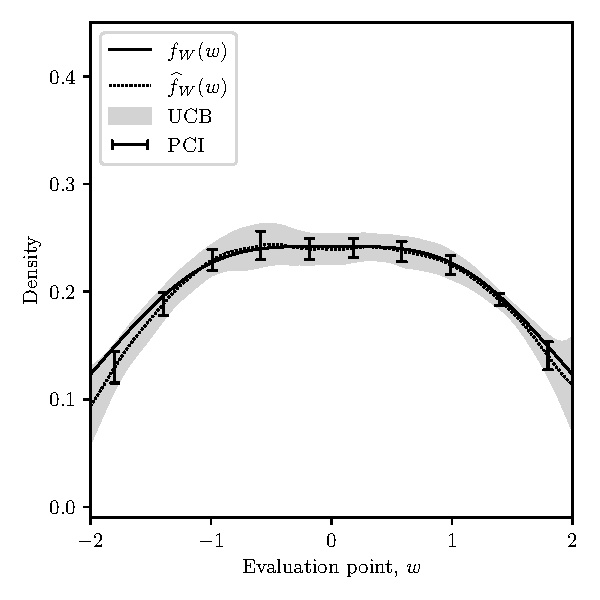
\includegraphics[scale=0.48]{graphics/result_total.pdf}
    \caption{
      Total degeneracy, \\
      $\pi = \left( \frac{1}{2}, 0, \frac{1}{2} \right)$
    }
  \end{subfigure}
  %
  \begin{subfigure}{0.32\textwidth}
    \centering
    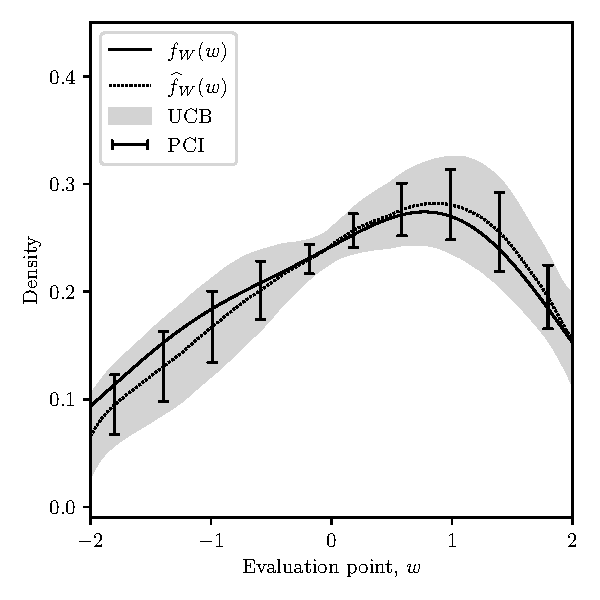
\includegraphics[scale=0.48]{graphics/result_partial.pdf}
    \caption{
      Partial degeneracy, \\
      $\pi = \left( \frac{1}{4}, 0, \frac{3}{4} \right)$
    }
  \end{subfigure}
  %
  \begin{subfigure}{0.32\textwidth}
    \centering
    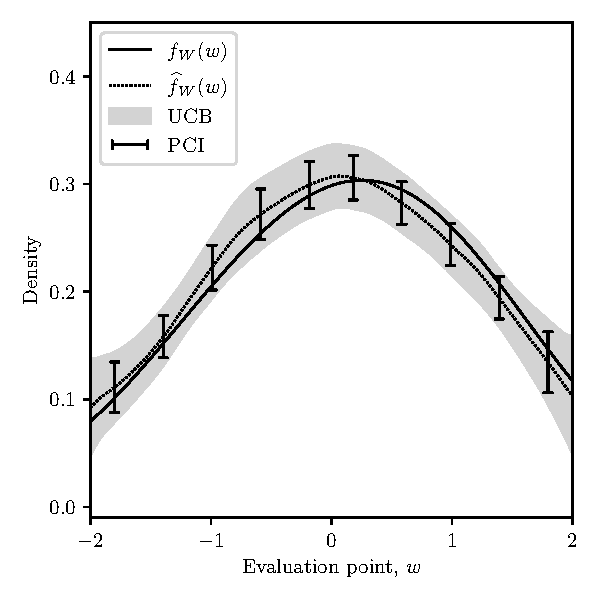
\includegraphics[scale=0.48]{graphics/result_none.pdf}
    \caption{
      No degeneracy, \\
      $\pi = \left( \frac{1}{5}, \frac{1}{5}, \frac{3}{5} \right)$
    }
  \end{subfigure}
  %
  \caption{
    Typical outcomes for three different values of the parameter $\pi$.
  }
  %
  \label{fig:results}
  %
  \vspace{-.8em}
\end{figure}

Next, Table~\ref{tab:results} presents numerical results.
For each degeneracy type (total, partial, none)
and each kernel order ($p=2$, $p=4$),
% four digit numbers do not need a space
we run $2000$ repeats
% four digit numbers do not need a space
with sample size $n=3000$ (giving $N=4\,498\,500$ pairs of nodes)
and with $d=50$ equally-spaced evaluation points.
We record the average rule-of-thumb bandwidth $\hat{h}_{\ROT}$
and the average root integrated mean squared error (RIMSE).
For both the uniform confidence bands (UCB)
and the pointwise confidence intervals (PCI),
we report the coverage rate (CR) and the average width (AW).
%
The lower-order kernel ($p=2$) ignores the bias, leading to
good RIMSE performance and acceptable UCB coverage
under partial or no degeneracy,
but gives invalid inference under total degeneracy.
In contrast, the higher-order kernel ($p=4$)
provides robust bias correction
and hence improves the coverage of the UCB in every regime,
particularly under total degeneracy,
at the cost of increasing both the RIMSE
and the average widths of the confidence bands.
%
As expected, the pointwise (in $w\in\cW$) confidence intervals (PCIs)
severely undercover in every regime.
Thus our simulation results show that the proposed feasible
inference methods based on robust bias correction and proper Studentization
deliver valid uniform inference
which is robust to unknown degenerate points
in the underlying dyadic distribution.

\begin{table}[ht]
  \caption{Numerical results for three values of the parameter $\pi$.}
  \vspace{-1em}
  \begin{center}
    \begin{tabular}{|c|c|c|c|c|cc|cc|}
      \hline
      \multirow{2}{*}{$ \pi $}
      & \multirow{2}{*}{Degeneracy type}
      & \multirow{2}{*}{$ \hat h_{\ROT} $}
      & \multirow{2}{*}{$ p $}
      & \multirow{2}{*}{RIMSE}
      & \multicolumn{2}{|c|}{UCB}
      & \multicolumn{2}{|c|}{PCI} \\
      \cline{6-9}
      & & & &
      & CR & AW
      & CR & AW \\
      \hline
      \multirow{2}{*}{$ \left(\frac{1}{2}, 0, \frac{1}{2}\right) $}
      & \multirow{2}{*}{Total}
      & \multirow{2}{*}{0.161}
      & 2 & 0.00048 & 87.1\% & 0.0028 & 6.5\% & 0.0017 \\
      & &  & 4 & 0.00068 & 95.2\% & 0.0042 & 9.7\% & 0.0025 \\
      \hline
      \multirow{2}{*}{$ \left(\frac{1}{4}, 0, \frac{3}{4}\right) $}
      & \multirow{2}{*}{Partial}
      & \multirow{2}{*}{0.158}
      & 2 & 0.00228 & 94.5\% & 0.0112 & 75.6\% & 0.0083 \\
      & &  & 4 & 0.00234 & 94.7\% & 0.0124 & 65.3\% & 0.0087 \\
      \hline
      \multirow{2}{*}{$ \left(\frac{1}{5}, \frac{1}{5}, \frac{3}{5}\right) $}
      & \multirow{2}{*}{None}
      & \multirow{2}{*}{0.145}
      & 2 & 0.00201 & 94.2\% & 0.0106 & 73.4\% & 0.0077 \\
      & &  & 4 & 0.00202 & 95.6\% & 0.0117 & 64.3\% & 0.0080 \\
      \hline
    \end{tabular}
  \end{center}
  % n = 3000
  % evaluation points = 50
  % repeats = 2000
  % resample = 10000
  \label{tab:results}
\end{table}

\section{Application: counterfactual dyadic density estimation}
\label{sec:counterfactual}

To further showcase the applicability of our main results,
we develop a kernel density estimator for
dyadic counterfactual distributions.
The aim of such counterfactual analysis is to estimate the
distribution of an outcome variable had some covariates
followed a distribution different from the actual one,
and it is important in causal inference and program evaluation settings
\citep{dinardo1996distribution,chernozhukov2013inference}.

For each $r \in \{0,1\}$,
let $\bW_n^r$, $\bA_n^r$ and $\bV_n^r$ be random variables
as defined in Assumption~\ref{ass:kernel_data} and
$\bX_n^r = (X_1^r, \ldots, X_n^r)$ be some covariates.
We assume that $(A_i^r, X_i^r)$ are
independent over $1 \leq i \leq n$
and that $\bX_n^r$ is independent of $\bV_n^r$,
that $W_{i j}^r \mid X_i^r, X_j^r$
has a conditional Lebesgue density
$f_{W \mid XX}^r(\,\cdot \mid x_1, x_2) \in \cH^\beta_{\CH}(\cW)$,
that $X_i^r$ follows a distribution function $F_X^r$
on a common support $\cX$, and that
$(\bA_n^0, \bV_n^0, \bX_n^0)$
is independent of $(\bA_n^1, \bV_n^1, \bX_n^1)$.

We interpret $r$ as an index for two populations,
labeled $0$ and $1$.
The counterfactual density of the outcome of
population $1$ had it followed the same covariate distribution
as population $0$ is
%
\begin{align*}
  f_W^{1 \triangleright 0}(w)
  &=
  \E\left[
    f_{W \mid XX}^1\big(w \mid X_1^0, X_2^0\big)
  \right] \\
  &=
  \int_{\cX}
  \int_{\cX}
  f_{W \mid XX}^{1}(w \mid x_1, x_2)
  \psi(x_1)
  \psi(x_2)
  \diff F_X^{1}(x_1)
  \diff F_X^{1}(x_2),
\end{align*}
%
where $\psi(x) = \mathrm{d} F_X^0(x) / \mathrm{d} F_X^1(x)$ for $x \in \cX$
is a Radon--Nikodym derivative.
If $X^0_i$ and $X^1_i$ have Lebesgue densities,
it is natural to consider a parametric model of the form
$\mathrm{d} F_X^{r}(x)=f_X^r(x;\theta)\diff x$
for some finite-dimensional parameter $\theta$.
Alternatively, if the covariates $X_n^r$ are discrete and have a positive
probability mass function $p_X^r(x)$ on a finite
support $\cX$, the object of interest becomes
$f_W^{1 \triangleright 0}(w)
= \sum_{x_1 \in \cX} \sum_{x_2 \in \cX}
f_{W \mid XX}^{1}(w \mid x_1, x_2) \psi(x_1) \psi(x_2)
p_X^{1}(x_1) p_X^{1}(x_2)$,
where $\psi(x) = p_X^0(x)/p_X^1(x)$ for $x \in \cX$.
We consider discrete covariates for simplicity,
and hence the counterfactual dyadic kernel density estimator is
%
\begin{align*}
  \hat f_W^{\,1 \triangleright 0}(w)
  &=
  \frac{2}{n(n-1)}
  \sum_{i=1}^{n-1}
  \sum_{j=i+1}^n
  \hat \psi(X_i^1)
  \hat \psi(X_j^1)
  k_h(W_{i j}^1, w),
\end{align*}
%
where $\hat\psi(x) = \hat p_X^{\,0}(x) / \hat p_X^{\,1}(x)$ and
$\hat p_X^{\,r}(x) = \frac{1}{n}\sum_{i = 1}^n \I\{X_i^r = x\}$,
with $\I$ the indicator function.

Section~SA2.10 of the online supplemental appendix provides technical details:
we show how an asymptotic
linear representation for $\hat\psi(x)$ leads to a
Hoeffding-type decomposition of $\hat f_W^{\,1 \triangleright 0}(w)$,
which is then used to establish that $\hat f_W^{\,1 \triangleright 0}$
is uniformly consistent for $f_W^{\,1 \triangleright 0}(w)$
and also admits a Gaussian strong approximation,
with the same rates of convergence
as for the standard density estimator.
Furthermore, define the covariance function of
$\hat f_W^{\,1 \triangleright 0}(w)$ as
$\Sigma_n^{1 \triangleright 0}(w,w') = \Cov\big[
  \hat f_W^{\,1 \triangleright 0}(w),
\hat f_W^{\,1 \triangleright 0}(w') \big]$,
which can be estimated as follows.
First let
$\hat\kappa(X_i^0, X_i^1, x)
= \frac{\I\{X_i^0 = x\} - \hat p_X^0(x)}{\hat p_X^1(x)}
- \frac{\hat p_X^0(x)}{\hat p_X^1(x)} \frac{\I\{X_i^1 = x\} - \hat
p_X^1(x)}{\hat p_X^1(x)}$
be a plug-in estimate of the influence function for $\hat\psi(x)$
and define the leave-one-out
conditional expectation estimators\newline
$S_i^{1 \triangleright 0}(w)
= \frac{1}{n-1} \big( \sum_{j=1}^{i-1} k_h(W_{j i}^1,w) \hat\psi(X_j^1)
+ \sum_{j=i+1}^n k_h(W_{i j}^1,w) \hat\psi(X_j^1) \big)$
and\newline
$\tilde S_i^{1 \triangleright 0}(w)
= \frac{1}{n-1} \sum_{j=1}^n \I\{j \neq i\}
\hat\kappa(X_i^0, X_i^1, X_j^1) S_j^{1 \triangleright 0}(w)$.
Then define the covariance estimator
%
\begin{align*}
  \hat\Sigma_n^{1 \triangleright 0}(w,w')
  &=
  \frac{4}{n^2}
  \sum_{i=1}^n
  \big(
    \hat\psi(X_i^1)
    S_i^{1 \triangleright 0}(w)
    + \tilde S_i^{1 \triangleright 0}(w)
  \big)
  \big(
    \hat\psi(X_i^1)
    S_i^{1 \triangleright 0}(w')
    + \tilde S_i^{1 \triangleright 0}(w')
  \big) \\
  &\quad-
  \frac{4}{n^3(n-1)}
  \sum_{i<j}
  k_h(W_{i j}^1, w)
  k_h(W_{i j}^1, w')
  \hat\psi(X_i^1)^2
  \hat\psi(X_j^1)^2
  - \frac{4}{n}
  \hat f_W^{\,1 \triangleright 0}(w)
  \hat f_W^{\,1 \triangleright 0}(w').
\end{align*}
%
We use a positive semi-definite approximation to
$\hat\Sigma_n^{1 \triangleright 0}$, denoted by
$\hat\Sigma_n^{+, 1 \triangleright 0}$,
as in Section~\ref{sec:covariance_estimation}.
To construct feasible uniform confidence bands,
define a process $\hat Z_n^{T, 1 \triangleright 0}(w)$ which
is conditionally mean-zero and Gaussian
given the data $\bW_n^1$, $\bX_n^0$ and $\bX_n^1$
and whose conditional covariance structure is
$\E\big[\hat Z_n^{T, 1 \triangleright 0}(w)
  \hat Z_n^{T, 1 \triangleright 0}(w')
\bigm| \bW_n^1, \bX_n^0, \bX_n^1 \big]
= \frac{\hat \Sigma_n^{+, 1 \triangleright 0}(w,w')}
{\sqrt{\hat \Sigma_n^{+, 1 \triangleright 0}(w,w)
\hat \Sigma_n^{+, 1 \triangleright 0}(w',w')}}$.
For $\alpha \in (0,1)$, define
$\hat q_{1-\alpha}^{\,1 \triangleright 0}$
as the conditional quantile satisfying
$\P\big(\sup_{w \in \cW}\big| \hat Z_n^{T, 1 \triangleright 0}(w) \big|
  \leq \hat q_{1-\alpha}^{\,1 \triangleright 0}
\bigm\vert \bW_n^1, \bX_n^0, \bX_n^1 \big)
= 1 - \alpha$.
Then, assuming that the covariance estimator is appropriately consistent,
%
\begin{align*}
  \P\left(
    f_W^{1 \triangleright 0}(w)
    \in
    \left[
      \hat f_W^{\,1 \triangleright 0}(w)
      \pm
      \hat q^{\,1 \triangleright 0}_{1-\alpha}
      \sqrt{\hat\Sigma_n^{+, 1 \triangleright 0}(w,w)}
    \,\right]
    \,\textup{for all }
    w \in \cW
  \right)
  \to 1 - \alpha,
\end{align*}
%
giving feasible uniform inference methods,
which are robust to unknown degeneracies,
for counterfactual distribution analysis in dyadic data settings.

\subsection{Application to trade data}
\label{sec:trade_data}

We illustrate the performance of our
estimation and inference methods with a real-world data set.
We use international bilateral trade data
from the International Monetary Fund's
Direction of Trade Statistics (DOTS),
previously analyzed by \citet{head2014gravity}
and \citet{chiang2022inference}.
This data set contains information about
the yearly trade flows among
$n = 207$ economies ($N = 21\,321$ pairs),
and we focus on the years
$1995$, $2000$ and $2005$.

We define the \emph{trade volume} between countries
$i$ and $j$ as the logarithm of the sum of
the trade flow (in billions of US dollars)
from $i$ to $j$
and the trade flow from $j$ to $i$.
In each year several pairs of countries
did not trade directly, yielding trade flows of zero
and hence a trade volume of $-\infty$.
We therefore assume that the distribution of trade volumes
is a mixture of a point mass at $-\infty$ and a
Lebesgue density on $\R$.
The local nature of our estimator means that
observations taking the value of $-\infty$
can simply be removed from the data set.
Table~\ref{tab:trade_network_stats}
gives summary statistics for these trade networks,
and shows how the networks tend to become more connected over time,
with edge density, average degree and clustering coefficient
all increasing.
%
%
%
%
\begin{table}[ht]
  \caption{Summary statistics for the DOTS trade networks.}
  \label{tab:trade_network_stats}
  \vspace{-1em}
  \begin{center}
    \begin{tabular}{|c|c|c|c|c|c|}
      \hline
      Year
      & Nodes
      & Edges
      & Edge density
      & Average degree
      & Clustering coefficient \\
      \hline
      1995 & 207 & 11\,603 & 0.5442 & 112.1 & 0.7250 \\
      2000 & 207 & 12\,528 & 0.5876 & 121.0 & 0.7674 \\
      2005 & 207 & 12\,807 & 0.6007 & 123.7 & 0.7745 \\
      \hline
    \end{tabular}
  \end{center}
  \vspace{-2em}
\end{table}

For counterfactual analysis we use the
gross domestic product (GDP) of each country as a
covariate, using $10\%$-percentiles to group the values into
$10$ different levels for ease of estimation.
This allows for a comparison of the observed distribution of trade at each year
with, for example, the counterfactual distribution of trade
had the GDP distribution remained as it was in $1995$.
As such we can measure how much of the change in trade
distribution is attributable
to a shift in the GDP distribution.

To estimate the trade volume density function
we use Algorithm~\ref{alg:method}
with $d=100$ equally-spaced evaluation points in $[-10,10]$,
using the rule-of-thumb bandwidth selector $\hat h_{\ROT}$
from Section~\ref{sec:bandwidth_selection} with
$p=2$ and $C(K) = 2.435$.
For inference we use an
Epanechnikov kernel of order $p=4$ and
resample the Gaussian process
$B = 10\,000$ times.
We also estimate the counterfactual trade distributions
in 2000 and 2005 respectively,
replacing the GDP distribution with that from 1995.
For each year, Figure~\ref{fig:trade}
plots the real and counterfactual density estimates
along with their respective uniform confidence bands (UCB)
at the nominal coverage rate of $95\%$.
Our empirical results show that
the counterfactual distribution drifts further from the truth
in 2005 compared with 2000, indicating a more significant shift
in the GDP distribution.
In the online supplemental appendix we repeat the procedure
using a parametric (log-normal maximum likelihood) preliminary estimate
of the GDP distribution, and observe that the results
are qualitatively similar.

\begin{figure}[ht]
  \centering
  %
  \begin{subfigure}{0.32\textwidth}
    \centering
    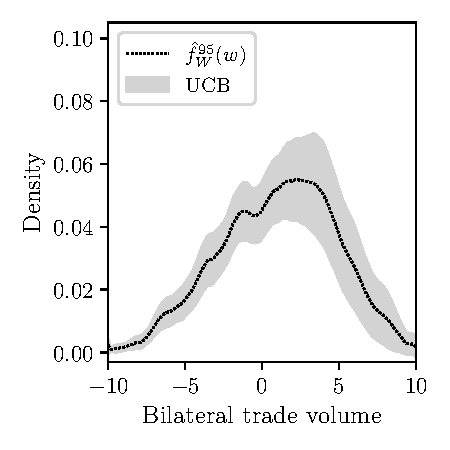
\includegraphics[scale=0.48]{graphics/trade_plot_1995.pdf}
    \caption{Year 1995, $\hat h_{\ROT} = 1.27$}
  \end{subfigure}
  %
  \begin{subfigure}{0.32\textwidth}
    \centering
    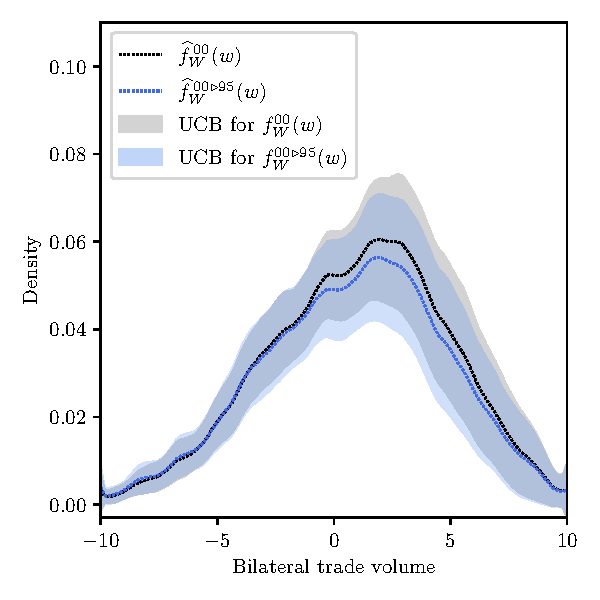
\includegraphics[scale=0.48]{graphics/trade_plot_1995_2000.pdf}
    \caption{Year 2000, $\hat h_{\ROT} = 1.31$}
  \end{subfigure}
  %
  \begin{subfigure}{0.32\textwidth}
    \centering
    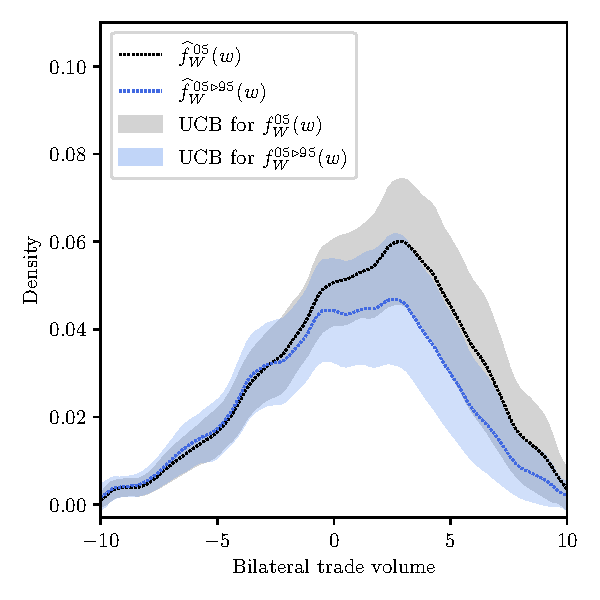
\includegraphics[scale=0.48]{graphics/trade_plot_1995_2005.pdf}
    \caption{Year 2005, $\hat h_{\ROT} = 1.37$}
  \end{subfigure}
  %
  \caption{Real and counterfactual density estimates
  and confidence bands for the DOTS data.}
  %
  \label{fig:trade}
  %
  % \vspace{-.8em}
  % \flushleft\footnotesize\emph{Notes}.
  % notes.
\end{figure}

\section{Other applications and future work}
\label{sec:future}

To emphasize the broad applicability of our methods
to network science problems,
we present three application scenarios.
The first concerns comparison of networks
\citep{kolaczyk2009statistical},
while the second and third involve
nonparametric and semiparametric dyadic regression
respectively.

Firstly, consider the setting where there are
two independent networks with
continuous dyadic covariates $\bW_n^0$ and $\bW_m^1$ respectively.
Practitioners may wish to test if these two dyadic distributions
are the same, that is, whether their density functions
$f_W^0$ and $f_W^1$ are equal on their
common support $\cW \subseteq \R$.
We present a family of hypothesis tests for this scenario
based on dyadic kernel density estimation.
Let $\hat f_W^{\,0}(w)$ and $\hat f_W^{\,1}(w)$
be the associated
(bias-corrected) dyadic kernel density estimators.
Consider the test statistics
$\tau_p$ for $1 \leq p \leq \infty$ where
%
\begin{align}
  \label{eq:hypothesis_test}
  \tau_p
  &=
  \left(
    \int_{-\infty}^{\infty}
    \left|
    \hat f_W^{\,1}(w)
    - \hat f_W^{\,0}(w)
    \right|^p
    \diff w
  \right)^{1/p}
  \text{ for } p < \infty, \text{ and }\,
  \tau_\infty
  = \sup_{w \in \cW}
  \left|
  \hat f_W^{\,1}(w)
  - \hat f_W^{\,0}(w)
  \right|.
\end{align}
%
Clearly we should reject the null hypothesis that $f_W^0 = f_W^1$ whenever
the test statistic $\tau_p$ is sufficiently large.
To estimate the critical value, let
$\hat\Sigma_n^{+,0}(w, w')$ and $\hat\Sigma_m^{+,1}(w, w')$
be the positive semi-definite estimators defined in
Section~\ref{sec:covariance_estimation} and
let $\hat Z^0_n(w)$ and $\hat Z^1_m(w)$ be zero-mean
Gaussian processes with covariance
structures $\hat\Sigma_n^{+,0}(w, w')$
and $\hat\Sigma_m^{+,1}(w, w')$
respectively, which are independent conditional on the data.
Define the approximate null test statistic
$\hat \tau_p$ by replacing
$\hat f_W^{\,0}(w)$ and $\hat f_W^{\,1}(w)$
with $\hat Z^0_n(w)$ and $\hat Z^1_m(w)$ respectively
in \eqref{eq:hypothesis_test}.
For a significance level $\alpha \in (0,1)$,
the critical value is $\hat C_\alpha$ where
%
$\P \big(
  \hat \tau_p \geq \hat C_\alpha \bigm\vert \bW_n^0, \bW_n^1
\big) = \alpha$.
%
This is estimated by Monte Carlo simulation, resampling
from the conditional law of
$\hat Z^0_n(w)$ and $\hat Z^1_m(w)$
and replacing integrals and suprema by sums and maxima over a
finite partition of $\cW$.

While our focus has been on density estimation with dyadic data,
our uniform dyadic estimation and inference results are readily
applicable to the settings of nonparametric
and semiparametric dyadic regression.
For a second example, suppose $Y_{i j} = Y(X_i, X_j, A_i, A_j, V_{i j})$,
where only $\bX_n$ and $\bY_n$ are observed and
$\bV_n$ is independent of $(\bX_n, \bA_n)$,
with $\bX_n = (X_i : 1 \leq i \leq n)$,
$\bA_n = (A_i : 1 \leq i \leq n)$,
$\bY_n = (Y_{i j}:1\leq i<j\leq n)$
and $\bV_n = (V_{i j} : 1 \leq i < j \leq n)$.
A parameter of interest is the regression function
$\mu(x_1, x_2) = \E[Y_{i j} \mid X_i=x_1, X_j=x_2]$,
which can be used to analyze average or partial effects
of changing the node attributes $X_i$ and $X_j$
on the edge variable $Y_{i j}$.
This conditional expectation could be estimated
using local polynomial methods:
suppose that $X_i$ takes values in $\R^m$ and
let $r(x_1, x_2)$ be a monomial basis up to degree
$\gamma \geq 0$ on $\R^m \times \R^m$. Then,
for some bandwidth $h > 0$ and
a kernel function $k_h$ on $\R^m \times \R^m$,
the local polynomial regression estimator of
$\mu(x_1, x_2)$ is
$\hat\mu(x_1, x_2)
= e_1^\T \hat\beta(x_1, x_2)$ where
$e_1$ is the first standard
unit vector in $\R^q$ for $q=\binom{2m+\gamma}{\gamma}$ and
\begin{align}
  \nonumber
  \hat{\beta}(x_1, x_2)
  &=
  \argmin_{\beta \in \R^q}
  \sum_{i=1}^{n-1}
  \sum_{j=i+1}^n
  \left(
    Y_{i j} - r(X_i-x_1, X_j-x_2)^\T \beta
  \right)^2
  k_h(X_i-x_1, X_j-x_2) \\
  \label{eq:locpol}
  &=
  \left(
    \sum_{i=1}^{n-1}
    \sum_{j=i+1}^n
    k_{i j} r_{i j} r_{i j}^\T
  \right)^{-1}
  \left(
    \sum_{i=1}^{n-1}
    \sum_{j=i+1}^n
    k_{i j} r_{i j} Y_{i j}
  \right),
\end{align}
with $k_{i j} = k_h(X_i-x_1, X_j-x_2)$
and
$r_{i j} = r(X_i-x_1, X_j-x_2)$.
\citet{graham2021dyadicregression}
established pointwise distribution theory
for the special case of the dyadic Nadaraya--Watson
kernel regression estimator ($\gamma=0$), but no uniform analogues
have yet been given.
It can be shown that the
``denominator'' matrix
in \eqref{eq:locpol} converges uniformly
to its expectation,
while the U-process-like ``numerator'' matrix
can be handled the same way as we analyzed
$\hat f_W(w)$ in this paper,
through a Hoeffding-type decomposition and
strong approximation methods,
along with standard bias calculations.
Such distributional approximation results can be used to construct valid
uniform confidence bands for the regression
function $\mu(x_1, x_2)$,
as well as to conduct hypothesis testing for
parametric specifications or shape constraints.

As a third example, we consider applying our results to
semiparametric semi-linear regression problems.
The dyadic semi-linear regression model is
%
$\E[Y_{i j} \mid W_{i j}, X_i, X_j]
= \theta^\T W_{i j} + g(X_i, X_j)$
%
where $\theta$ is the finite-dimensional parameter
of interest
and $g(X_i, X_j)$ is an unknown
function of the covariates
$(X_i, X_j)$.
Local polynomial (or other) methods can be used to
estimate $\theta$ and $g$,
where the estimator of the nonparametric component
$g$ takes a similar form to \eqref{eq:locpol},
that is, a ratio of two kernel-based
estimators as in \eqref{eq:kernel_estimator}.
Consequently, our strong approximation techniques
presented in this paper can be appropriately modified
to develop valid uniform inference procedures for
$g$ and $\E[Y_{i j} \mid W_{i j}=w, X_i=x_1, X_j=x_2]$,
as well as functionals thereof.

\section{Conclusion}
\label{sec:conclusion}

We studied the uniform estimation and inference properties of the
dyadic kernel density estimator
$\hat{f}_W$ given in \eqref{eq:kernel_estimator},
which forms a class
of U-process-like estimators
indexed by the $n$-varying kernel function $k_h$ on $\cW$.
We established uniform minimax-optimal point estimation results
and uniform distributional approximations for this estimator
based on novel strong approximation strategies.
We then applied these results to derive valid
and feasible uniform confidence bands for
the dyadic density estimand $f_W$,
and also developed a substantive application of our theory to
counterfactual dyadic density analysis.
We gave some other statistical
applications of our methodology as well as
potential avenues for future research.
From a technical perspective,
the online supplemental appendix contains several generic results
concerning strong approximation methods and maximal inequalities
for empirical processes that may be of independent interest.
This work has been presented as
%
\cite{%
  cattaneo2022talkgeorgia,%
  cattaneo2022talkcolumbia,%
  feng2022talkrenmin,%
  feng2022talkxiamen,%
  feng2023talkpeking,%
  feng2023talksingapore%
}.
